\documentclass[output=book
		,modfonts
		,nonflat
	        ,collection
	        ,collectionchapter
	        ,collectiontoclongg
 	        ,biblatex  
                ,babelshorthands
%                ,showindex
                ,newtxmath
                ,colorlinks, citecolor=brown 
                ,draftmode
% 	        ,coverus
		  ]{langscibook}                              
%%%%%%%%%%%%%%%%%%%%%%%%%%%%%%%%%%%%%%%%%%%%%%%%%%%%

% put all additional commands you need in the 
% following files. If you do not know what this might 
% mean, you can safely ignore this section

\title{Head-Driven Phrase Structure Grammar}  %look no further, you can change those things right here.
\subtitle{The handbook}
% \BackTitle{Change your backtitle in localmetadata.tex} % Change if BackTitle != Title
\BackBody{Head-Driven Phrase Structure Grammar (HPSG) is a linguistic framework that models
  linguistic knowledge on all descriptive levels (phonology, morphology, syntax, semantics,
  pragmatics) by using feature value pairs, structure sharing, and relational constraints. This
  volume summarizes work that has been done since the mid 80s. Various chapters discus formal foundations and
  basic assumptions, describe the evolution of the framework and go into the details of various
  syntactic phenomena. Separate chapters are devoted to non-syntactic levels of description. The
  book also handles related fields and research areas (gesture, sign languages, computational
  linguistics) and has a part in which HPSG is compared to other frameworks (Lexical Functional
  Grammar, Categorial Grammar, Construction Grammar, Dependency Grammar and Minimalim).    
 }
%\dedication{Change dedication in localmetadata.tex}
\typesetter{Stefan Müller, Elizabeth Pankratz}
\proofreader{Elizabeth Pankratz}
\author{Stefan Müller\and Anne Abeillé\and Robert D. Borsley\lastand Jean-​Pierre Koenig}
% \BookDOI{}%ask coordinator for DOI
\renewcommand{\lsISBNdigital}{978-3-96110-255-6}
\renewcommand{\lsISBNhardcover}{000-0-000000-00-0}
\renewcommand{\lsISBNsoftcover}{000-0-000000-00-0}
\renewcommand{\lsISBNsoftcoverus}{000-0-000000-00-0}
\renewcommand{\lsSeries}{eotms} % use lowercase acronym, e.g. sidl, eotms, tgdi
\renewcommand{\lsSeriesNumber}{} %will be assigned when the book enters the proofreading stage
% \renewcommand{\lsURL}{http://langsci-press.org/catalog/book/000} % contact the coordinator for the right number

% add all extra packages you need to load to this file 

% the ISBN assigned to the digital edition
\usepackage[ISBN=9783961102556]{ean13isbn} 

\usepackage{graphicx}
\usepackage{tabularx}
\usepackage{amsmath} 

%\usepackage{tipa}      % Davis Koenig
\usepackage{xunicode} % Provide tipa macros (BC)

\usepackage{multicol}

% Berthold morphology
\usepackage{relsize}
%\usepackage{./styles/rtrees-bc} % forbidden forest 08.12.2019


\usepackage{langsci-optional} 
% used to be in this package
\providecommand{\citegen}{}
\renewcommand{\citegen}[2][]{\citeauthor{#2}'s (\citeyear*[#1]{#2})}
\providecommand{\lsptoprule}{}
\renewcommand{\lsptoprule}{\midrule\toprule}
\providecommand{\lspbottomrule}{}
\renewcommand{\lspbottomrule}{\bottomrule\midrule}
\providecommand{\largerpage}{}
\renewcommand{\largerpage}[1][1]{\enlargethispage{#1\baselineskip}}


\usepackage{langsci-lgr}

\newcommand{\MAS}{\textsc{m}\xspace} % \M is taken by somebody

%\usepackage{./styles/forest/forest}
\usepackage{langsci-forest-setup}

\usepackage{./styles/memoize/memoize} 
\memoizeset{
  memo filename prefix={chapters/hpsg-handbook.memo.dir/},
  register=\todo{O{}+m},
  prevent=\todo,
}

\usepackage{tikz-cd}

\usepackage{./styles/tikz-grid}
\usetikzlibrary{shadows}


% removed with texlive 2020 06.05.2020
% %\usepackage{pgfplots} % for data/theory figure in minimalism.tex
% % fix some issue with Mod https://tex.stackexchange.com/a/330076
% \makeatletter
% \let\pgfmathModX=\pgfmathMod@
% \usepackage{pgfplots}%
% \let\pgfmathMod@=\pgfmathModX
% \makeatother

\usepackage{subcaption}

% Stefan Müller's styles
\usepackage{./styles/merkmalstruktur,german,./styles/makros.2020,./styles/my-xspace,./styles/article-ex,
./styles/eng-date}

\selectlanguage{USenglish}

\usepackage{./styles/abbrev}


% Has to be loaded late since otherwise footnotes will not work

%%%%%%%%%%%%%%%%%%%%%%%%%%%%%%%%%%%%%%%%%%%%%%%%%%%%
%%%                                              %%%
%%%           Examples                           %%%
%%%                                              %%%
%%%%%%%%%%%%%%%%%%%%%%%%%%%%%%%%%%%%%%%%%%%%%%%%%%%%
% remove the percentage signs in the following lines
% if your book makes use of linguistic examples
\usepackage{langsci-gb4e} 


%% St. Mü.: 03.04.2020
%% these two versions of the command can be used for series of sets of examples:
%% \eal
%% \ex
%% \ex
%% \zlcont
%% \ealcont
%% \ex
%% \ex
%% \zl

\let\zlcont\z
\def\ealcont{\exnrfont\ex\begin{xlist}[iv.]\raggedright}

% original version of \z
%\def\z{\ifnum\@xnumdepth=1\end{exe}\else\end{xlist}\fi}
% \zcont just removes \end{exe}
%\def\zcont{\ifnum\@xnumdepth=1\else\end{xlist}\fi}
\def\zcont{}

% Crossing out text
% uncomment when needed
%\usepackage{ulem}

\usepackage{./styles/additional-langsci-index-shortcuts}

% this is the completely redone avm package
\usepackage{./styles/langsci-avm}
\avmsetup{columnsep=.3ex,style=narrow}

%\let\asort\type*


\usepackage{./styles/avm+}


\renewcommand{\tpv}[1]{{\avmjvalfont\itshape #1}}

% no small caps please
\renewcommand{\phonshape}[0]{\normalfont\itshape}

\regAvmFonts

\usepackage{theorem}

\newtheorem{mydefinition}{Def.}
\newtheorem{principle}{Principle}

{\theoremstyle{break}
%\newtheorem{schema}{Schema}
\newtheorem{mydefinition-break}[mydefinition]{Def.}
\newtheorem{principle-break}[principle]{Principle}
}


%% \newcommand{schema}[2]{
%% \begin{minipage}{\textwidth}
%% {\textbf{Schema~\theschema}}]\hspace{.5em}\textbf{(#1)}\\
%% #2
%% \end{minipage}}


% This avoids linebreaks in the Schema
\newcounter{schemacounter}
\makeatletter
\newenvironment{schema}[1][]
  {%
   \refstepcounter{schemacounter}%
   \par\bigskip\noindent
   \minipage{\linewidth}%
   \textbf{Schema~\theschemacounter\hspace{.5em} \ifx&#1&\else(#1)\fi}\par
  }{\endminipage\par\bigskip\@endparenv}%
\makeatother

%\usepackage{subfig}





% Davis Koenig Lexikon

\usepackage{tikz-qtree,tikz-qtree-compat} % Davis Koenig remove

\usepackage{shadow}



\usepackage[english]{isodate} % Andy Lücking
\usepackage[autostyle]{csquotes} % Andy
%\usepackage[autolanguage]{numprint}

%\defaultfontfeatures{
%    Path = /usr/local/texlive/2017/texmf-dist/fonts/opentype/public/fontawesome/ }

%% https://tex.stackexchange.com/a/316948/18561
%\defaultfontfeatures{Extension = .otf}% adds .otf to end of path when font loaded without ext parameter e.g. \newfontfamily{\FA}{FontAwesome} > \newfontfamily{\FA}{FontAwesome.otf}
%\usepackage{fontawesome} % Andy Lücking
\usepackage{pifont} % Andy Lücking -> hand

\usetikzlibrary{decorations.pathreplacing} % Andy Lücking
\usetikzlibrary{matrix} % Andy 
\usetikzlibrary{positioning} % Andy
\usepackage{tikz-3dplot} % Andy

% pragmatics
\usepackage{eqparbox} % Andy
\usepackage{enumitem} % Andy
\usepackage{longtable} % Andy
\usepackage{tabu} % Andy              needs to be loaded before hyperref as of texlive 2020

% tabu-fix
% to make "spread 0pt" work
% -----------------------------
\RequirePackage{etoolbox}
\makeatletter
\patchcmd
	\tabu@startpboxmeasure
	{\bgroup\begin{varwidth}}%
	{\bgroup
	 \iftabu@spread\color@begingroup\fi\begin{varwidth}}%
	{}{}
\def\@tabarray{\m@th\def\tabu@currentgrouptype
    {\currentgrouptype}\@ifnextchar[\@array{\@array[c]}}
%
%%% \pdfelapsedtime bug 2019-12-15
\patchcmd
	\tabu@message@etime
	{\the\pdfelapsedtime}%
	{\pdfelapsedtime}%
	{}{}
%
%
\makeatother
% -----------------------------


% Manfred's packages

%\usepackage{shadow}

\usepackage{tabularx}
\newcolumntype{L}[1]{>{\raggedright\arraybackslash}p{#1}} % linksbündig mit Breitenangabe


% Jong-Bok

%\usepackage{xytree}

\newcommand{\xytree}[2][dummy]{Let's do the tree!}

% seems evil, get rid of it
% defines \ex is incompatible with gb4e
%\usepackage{lingmacros}

% taken from lingmacros:
\makeatletter
% \evnup is used to line up the enumsentence number and an entry along
% the top.  It can take an argument to improve lining up.
\def\evnup{\@ifnextchar[{\@evnup}{\@evnup[0pt]}}

\def\@evnup[#1]#2{\setbox1=\hbox{#2}%
\dimen1=\ht1 \advance\dimen1 by -.5\baselineskip%
\advance\dimen1 by -#1%
\leavevmode\lower\dimen1\box1}
\makeatother


% YK -- CG chapter

%\usepackage{xspace}
\usepackage{bm}
\usepackage{ebproof}


% Antonio Branco, remove this
\usepackage{epsfig}

% now unicode
%\usepackage{alphabeta}





\usepackage{pst-node}


% fmr: additional packages
%\usepackage{amsthm}


% Ash and Steve: LFG
\usepackage{./styles/lfg/dalrymple}

\RequirePackage{graphics}
%\RequirePackage{./styles/lfg/trees}
%% \RequirePackage{avm}
%% \avmoptions{active}
%% \avmfont{\sc}
%% \avmvalfont{\sc}
\RequirePackage{./styles/lfg/lfgmacrosash}

\usepackage{./styles/lfg/glue}

%%%%%%%%%%%%%%%%%%%%%%%%%%%%%%
%% Markup
%%%%%%%%%%%%%%%%%%%%%%%%%%%%%%
\usepackage[normalem]{ulem} % For thinks like strikethrough, using \sout

% \newcommand{\high}[1]{\textbf{#1}} % highlighted text
\newcommand{\high}[1]{\textit{#1}} % highlighted text
%\newcommand{\term}[1]{\textit{#1}\/} % technical term
\newcommand{\qterm}[1]{`{#1}'} % technical term, quotes
%\newcommand{\trns}[1]{\strut `#1'} % translation in glossed example
\newcommand{\trnss}[1]{\strut \phantom{\sqz{}} `#1'} % translation in ungrammatical glossed example
\newcommand{\ttrns}[1]{(`#1')} % an in-text translation of a word
%\newcommand{\feat}[1]{\mbox{\textsc{\MakeLowercase{#1}}}}     % feature name
%\newcommand{\val}[1]{\mbox{\textsc{\MakeLowercase{#1}}}}    % f-structure value
\newcommand{\featt}[1]{\mbox{\textsc{\MakeLowercase{#1}}}}     % feature name
\newcommand{\vall}[1]{\mbox{\textsc{\textup{\MakeLowercase{#1}}}}}    % f-structure value
\newcommand{\mg}[1]{\mbox{\textsc{\MakeLowercase{#1}}}}    % morphological gloss
%\newcommand{\word}[1]{\textit{#1}}       % mention of word
\providecommand{\kstar}[1]{{#1}\ensuremath{^*}}
\providecommand{\kplus}[1]{{#1}\ensuremath{^+}}
\newcommand{\template}[1]{@\textsc{\MakeLowercase{#1}}}
\newcommand{\templaten}[1]{\textsc{\MakeLowercase{#1}}}
\newcommand{\templatenn}[1]{\MakeUppercase{#1}}
\newcommand{\tempeq}{\ensuremath{=}}
\newcommand{\predval}[1]{\ensuremath{\langle}\textsc{#1}\ensuremath{\rangle}}
\newcommand{\predvall}[1]{{\rm `#1'}}
\newcommand{\lfgfst}[1]{\ensuremath{#1\,}}
\newcommand{\scare}[1]{`#1'} % scare quotes
\newcommand{\bracket}[1]{\ensuremath{\left\langle\mathit{#1}\right\rangle}}
\newcommand{\sectionw}[1][]{Section#1} % section word: for cap/non-cap
\newcommand{\tablew}[1][]{Table#1} % table word: for cap/non-cap
\newcommand{\lfgglue}{LFG+Glue}
\newcommand{\hpsgglue}{HPSG+Glue}
\newcommand{\gs}{GS}
%\newcommand{\func}[1]{\ensuremath{\mathbf{#1}}}
\newcommand{\func}[1]{\textbf{#1}}
\renewcommand{\glue}{Glue}
%\newcommand{\exr}[1]{(\ref{ex:#1}}
\newcommand{\exra}[1]{(\ref{ex:#1})}


%%%%%%%%%%%%%%%%%%%%%%%%%%%%%%
% Notation
%\newcommand{\xbar}[1]{$_{\mbox{\textsc{#1}$^{\raisebox{1ex}{}}$}}$}
\newcommand{\xprime}[2][]{\textup{\mbox{{#2}\ensuremath{^\prime_{\hspace*{-.0em}\mbox{\footnotesize\ensuremath{\mathit{#1}}}}}}}}
\providecommand{\xzero}[2][]{#2\ensuremath{^0_{\mbox{\footnotesize\ensuremath{\mathit{#1}}}}}}



\let\leftangle\langle
\let\rightangle\rangle

%\newcommand{\pslabel}[1]{}



%% hyphenation points for line breaks
%% Normally, automatic hyphenation in LaTeX is very good
%% If a word is mis-hyphenated, add it to this file
%%
%% add information to TeX file before \begin{document} with:
%% %% hyphenation points for line breaks
%% Normally, automatic hyphenation in LaTeX is very good
%% If a word is mis-hyphenated, add it to this file
%%
%% add information to TeX file before \begin{document} with:
%% %% hyphenation points for line breaks
%% Normally, automatic hyphenation in LaTeX is very good
%% If a word is mis-hyphenated, add it to this file
%%
%% add information to TeX file before \begin{document} with:
%% \include{localhyphenation}
\hyphenation{
A-la-hver-dzhie-va
anaph-o-ra
ana-phor
ana-phors
an-te-ced-ent
an-te-ced-ents
affri-ca-te
affri-ca-tes
ap-proach-es
Atha-bas-kan
Athe-nä-um
Bona-mi
Chi-che-ŵa
com-ple-ments
con-straints
Cope-sta-ke
Da-ge-stan
Dor-drecht
er-klä-ren-de
Ginz-burg
Gro-ning-en
Jap-a-nese
Jon-a-than
Ka-tho-lie-ke
Ko-bon
krie-gen
Le-Sourd
moth-er
Mül-ler
Nie-mey-er
Par-a-digm
Prze-piór-kow-ski
phe-nom-e-non
re-nowned
Rie-he-mann
un-bound-ed
with-in
}

% listing within here does not have any effect for lfg.tex % 2020-05-14

% why has "erklärende" be listed here? I specified langid in bibtex item. Something is still not working with hyphenation.


% to do: check
%  Alahverdzhieva


% biblatex:

% This is a LaTeX frontend to TeX’s \hyphenation command which defines hy- phenation exceptions. The ⟨language⟩ must be a language name known to the babel/polyglossia packages. The ⟨text ⟩ is a whitespace-separated list of words. Hyphenation points are marked with a dash:

% \DefineHyphenationExceptions{american}{%
% hy-phen-ation ex-cep-tion }

\hyphenation{
A-la-hver-dzhie-va
anaph-o-ra
ana-phor
ana-phors
an-te-ced-ent
an-te-ced-ents
affri-ca-te
affri-ca-tes
ap-proach-es
Atha-bas-kan
Athe-nä-um
Bona-mi
Chi-che-ŵa
com-ple-ments
con-straints
Cope-sta-ke
Da-ge-stan
Dor-drecht
er-klä-ren-de
Ginz-burg
Gro-ning-en
Jap-a-nese
Jon-a-than
Ka-tho-lie-ke
Ko-bon
krie-gen
Le-Sourd
moth-er
Mül-ler
Nie-mey-er
Par-a-digm
Prze-piór-kow-ski
phe-nom-e-non
re-nowned
Rie-he-mann
un-bound-ed
with-in
}

% listing within here does not have any effect for lfg.tex % 2020-05-14

% why has "erklärende" be listed here? I specified langid in bibtex item. Something is still not working with hyphenation.


% to do: check
%  Alahverdzhieva


% biblatex:

% This is a LaTeX frontend to TeX’s \hyphenation command which defines hy- phenation exceptions. The ⟨language⟩ must be a language name known to the babel/polyglossia packages. The ⟨text ⟩ is a whitespace-separated list of words. Hyphenation points are marked with a dash:

% \DefineHyphenationExceptions{american}{%
% hy-phen-ation ex-cep-tion }

\hyphenation{
A-la-hver-dzhie-va
anaph-o-ra
ana-phor
ana-phors
an-te-ced-ent
an-te-ced-ents
affri-ca-te
affri-ca-tes
ap-proach-es
Atha-bas-kan
Athe-nä-um
Bona-mi
Chi-che-ŵa
com-ple-ments
con-straints
Cope-sta-ke
Da-ge-stan
Dor-drecht
er-klä-ren-de
Ginz-burg
Gro-ning-en
Jap-a-nese
Jon-a-than
Ka-tho-lie-ke
Ko-bon
krie-gen
Le-Sourd
moth-er
Mül-ler
Nie-mey-er
Par-a-digm
Prze-piór-kow-ski
phe-nom-e-non
re-nowned
Rie-he-mann
un-bound-ed
with-in
}

% listing within here does not have any effect for lfg.tex % 2020-05-14

% why has "erklärende" be listed here? I specified langid in bibtex item. Something is still not working with hyphenation.


% to do: check
%  Alahverdzhieva


% biblatex:

% This is a LaTeX frontend to TeX’s \hyphenation command which defines hy- phenation exceptions. The ⟨language⟩ must be a language name known to the babel/polyglossia packages. The ⟨text ⟩ is a whitespace-separated list of words. Hyphenation points are marked with a dash:

% \DefineHyphenationExceptions{american}{%
% hy-phen-ation ex-cep-tion }

%add all your local new commands to this file


% Don't do this at home. I do not like the smaller font for captions.
% I just removed loading the caption packege in langscibook.cls
%% \captionsetup{%
%% font={%
%% stretch=1%.8%
%% ,normalsize%,small%
%% },%
%% width=.8\textwidth
%% }

\makeatletter
\def\blx@maxline{77}
\makeatother


\newcommand{\page}{}

\newcommand{\todostefan}[1]{\todo[color=orange!80]{\footnotesize #1}\xspace}
\newcommand{\todosatz}[1]{\todo[color=red!40]{\footnotesize #1}\xspace}

\newcommand{\inlinetodostefan}[1]{\todo[color=green!40,inline]{\footnotesize #1}\xspace}

\newcommand{\addpages}{\todostefan{add pages}}
\newcommand{\addglosses}{\todostefan{add glosses}}


\newcommand{\spacebr}{\hspaceThis{[}}

\newcommand{\danish}{\jambox{(\ili{Danish})}}
\newcommand{\english}{\jambox{(\ili{English})}}
\newcommand{\german}{\jambox{(\ili{German})}}
\newcommand{\yiddish}{\jambox{(\ili{Yiddish})}}
\newcommand{\welsh}{\jambox{(\ili{Welsh})}}

% Cite and cross-reference other chapters
\newcommand{\crossrefchaptert}[2][]{\citet*[#1]{chapters/#2}, Chapter~\ref{chap-#2} of this volume} 
\newcommand{\crossrefchapterp}[2][]{(\citealp*[#1]{chapters/#2}, Chapter~\ref{chap-#2} of this volume)}
\newcommand{\crossrefchapteralt}[2][]{\citealt*[#1]{chapters/#2}, Chapter~\ref{chap-#2} of this volume}
\newcommand{\crossrefchapteralp}[2][]{\citealp*[#1]{chapters/#2}, Chapter~\ref{chap-#2} of this volume}
% example of optional argument:
% \crossrefchapterp[for something, see:]{name}
% gives: (for something, see: Author 2018, Chapter~X of this volume)

\let\crossrefchapterw\crossrefchaptert



% Davis Koenig

\let\ig=\textsc
\let\tc=\textcolor

% evolution, Flickinger, Pollard, Wasow

\let\citeNP\citet

% Adam P

%\newcommand{\toappear}{Forthcoming}
\newcommand{\pg}[1]{p.\,#1}
\renewcommand{\implies}{\rightarrow}

\newcommand*{\rref}[1]{(\ref{#1})}
\newcommand*{\aref}[1]{(\ref{#1}a)}
\newcommand*{\bref}[1]{(\ref{#1}b)}
\newcommand*{\cref}[1]{(\ref{#1}c)}

\newcommand{\msadam}{.}
\newcommand{\morsyn}[1]{\textsc{#1}}

\newcommand{\nom}{\morsyn{nom}}
\newcommand{\acc}{\morsyn{acc}}
\newcommand{\dat}{\morsyn{dat}}
\newcommand{\gen}{\morsyn{gen}}
\newcommand{\ins}{\morsyn{ins}}
%\newcommand{\aploc}{\morsyn{loc}}
\newcommand{\voc}{\morsyn{voc}}
\newcommand{\ill}{\morsyn{ill}}
\renewcommand{\inf}{\morsyn{inf}}
\newcommand{\passprc}{\morsyn{passp}}

%\newcommand{\Nom}{\msadam\nom}
%\newcommand{\Acc}{\msadam\acc}
%\newcommand{\Dat}{\msadam\dat}
%\newcommand{\Gen}{\msadam\gen}
\newcommand{\Ins}{\msadam\ins}
\newcommand{\Loc}{\msadam\loc}
\newcommand{\Voc}{\msadam\voc}
\newcommand{\Ill}{\msadam\ill}
\newcommand{\PassP}{\msadam\passprc}

\newcommand{\Aux}{\textsc{aux}}

\newcommand{\princ}[1]{\textnormal{\textsc{#1}}} % for constraint names
\newcommand{\notion}[1]{\emph{#1}}
\renewcommand{\path}[1]{\textnormal{\textsc{#1}}}
\newcommand{\ftype}[1]{\textit{#1}}
\newcommand{\fftype}[1]{{\scriptsize\textit{#1}}}
\newcommand{\la}{$\langle$}
\newcommand{\ra}{$\rangle$}
%\newcommand{\argst}{\path{arg-st}}
\newcommand{\phtm}[1]{\setbox0=\hbox{#1}\hspace{\wd0}}
\newcommand{\prep}[1]{\setbox0=\hbox{#1}\hspace{-1\wd0}#1}

%%%%%%%%%%%%%%%%%%%%%%%%%%%%%%%%%%%%%%%%%%%%%%%%%%%%%%%%%%%%%%%%%%%%%%%%%%%

% FROM FS.STY:

%%%
%%% Feature structures
%%%

% \fs         To print a feature structure by itself, type for example
%             \fs{case:nom \\ person:P}
%             or (better, for true italics),
%             \fs{\it case:nom \\ \it person:P}
%
% \lfs        To print the same feature structure with the category
%             label N at the top, type:
%             \lfs{N}{\it case:nom \\ \it person:P}

%    Modified 1990 Dec 5 so that features are left aligned.
\newcommand{\fs}[1]%
{\mbox{\small%
$
\!
\left[
  \!\!
  \begin{tabular}{l}
    #1
  \end{tabular}
  \!\!
\right]
\!
$}}

%     Modified 1990 Dec 5 so that features are left aligned.
%\newcommand{\lfs}[2]
%   {
%     \mbox{$
%           \!\!
%           \begin{tabular}{c}
%           \it #1
%           \\
%           \mbox{\small%
%                 $
%                 \left[
%                 \!\!
%                 \it
%                 \begin{tabular}{l}
%                 #2
%                 \end{tabular}
%                 \!\!
%                 \right]
%                 $}
%           \end{tabular}
%           \!\!
%           $}
%   }

\newcommand{\ft}[2]{\path{#1}\hspace{1ex}\ftype{#2}}
\newcommand{\fsl}[2]{\fs{{\fftype{#1}} \\ #2}}

\newcommand{\fslt}[2]
 {\fst{
       {\fftype{#1}} \\
       #2 
     }
 }

\newcommand{\fsltt}[2]
 {\fstt{
       {\fftype{#1}} \\
       #2 
     }
 }

\newcommand{\fslttt}[2]
 {\fsttt{
       {\fftype{#1}} \\
       #2 
     }
 }


% jak \ft, \fs i \fsl tylko nieco ciasniejsze

\newcommand{\ftt}[2]
% {{\sc #1}\/{\rm #2}}
 {\textsc{#1}\/{\rm #2}}

\newcommand{\fst}[1]
  {
    \mbox{\small%
          $
          \left[
          \!\!\!
%          \sc
          \begin{tabular}{l} #1
          \end{tabular}
          \!\!\!\!\!\!\!
          \right]
          $
          }
   }

%\newcommand{\fslt}[2]
% {\fst{#2\\
%       {\scriptsize\it #1}
%      }
% }


% superciasne

\newcommand{\fstt}[1]
  {
    \mbox{\small%
          $
          \left[
          \!\!\!
%          \sc
          \begin{tabular}{l} #1
          \end{tabular}
          \!\!\!\!\!\!\!\!\!\!\!
          \right]
          $
          }
   }

%\newcommand{\fsltt}[2]
% {\fstt{#2\\
%       {\scriptsize\it #1}
%      }
% }

\newcommand{\fsttt}[1]
  {
    \mbox{\small%
          $
          \left[
          \!\!\!
%          \sc
          \begin{tabular}{l} #1
          \end{tabular}
          \!\!\!\!\!\!\!\!\!\!\!\!\!\!\!\!
          \right]
          $
          }
   }



% %add all your local new commands to this file

% \newcommand{\smiley}{:)}

% you are not supposed to mess with hardcore stuff, St.Mü. 22.08.2018
%% \renewbibmacro*{index:name}[5]{%
%%   \usebibmacro{index:entry}{#1}
%%     {\iffieldundef{usera}{}{\thefield{usera}\actualoperator}\mkbibindexname{#2}{#3}{#4}{#5}}}

% % \newcommand{\noop}[1]{}



% Rui

\newcommand{\spc}[0]{\hspace{-1pt}\underline{\hspace{6pt}}\,}
\newcommand{\spcs}[0]{\hspace{-1pt}\underline{\hspace{6pt}}\,\,}
\newcommand{\bad}[1]{\leavevmode\llap{#1}}
\newcommand{\COMMENT}[1]{}


% Rui coordination
\newcommand{\subl}[1]{$_{\scriptstyle \textsc{#1}}$}



% Andy Lücking gesture.tex
\newcommand{\Pointing}{\ding{43}}
% Giotto: "Meeting of Joachim and Anne at the Golden Gate" - 1305-10 
\definecolor{GoldenGate1}{rgb}{.13,.09,.13} % Dress of woman in black
\definecolor{GoldenGate2}{rgb}{.94,.94,.91} % Bridge
\definecolor{GoldenGate3}{rgb}{.06,.09,.22} % Blue sky
\definecolor{GoldenGate4}{rgb}{.94,.91,.87} % Dress of woman with shawl
\definecolor{GoldenGate5}{rgb}{.52,.26,.26} % Joachim's robe
\definecolor{GoldenGate6}{rgb}{.65,.35,.16} % Anne's robe
\definecolor{GoldenGate7}{rgb}{.91,.84,.42} % Joachim's halo

\makeatletter
\newcommand{\@Depth}{1} % x-dimension, to front
\newcommand{\@Height}{1} % z-dimension, up
\newcommand{\@Width}{1} % y-dimension, rightwards
%\GGS{<x-start>}{<y-start>}{<z-top>}{<z-bottom>}{<Farbe>}{<x-width>}{<y-depth>}{<opacity>}
\newcommand{\GGS}[9][]{%
\coordinate (O) at (#2-1,#3-1,#5);
\coordinate (A) at (#2-1,#3-1+#7,#5);
\coordinate (B) at (#2-1,#3-1+#7,#4);
\coordinate (C) at (#2-1,#3-1,#4);
\coordinate (D) at (#2-1+#8,#3-1,#5);
\coordinate (E) at (#2-1+#8,#3-1+#7,#5);
\coordinate (F) at (#2-1+#8,#3-1+#7,#4);
\coordinate (G) at (#2-1+#8,#3-1,#4);
\draw[draw=black, fill=#6, fill opacity=#9] (D) -- (E) -- (F) -- (G) -- cycle;% Front
\draw[draw=black, fill=#6, fill opacity=#9] (C) -- (B) -- (F) -- (G) -- cycle;% Top
\draw[draw=black, fill=#6, fill opacity=#9] (A) -- (B) -- (F) -- (E) -- cycle;% Right
}
\makeatother


% pragmatics
\newcommand{\speaking}[1]{\eqparbox{name}{\textsc{\lowercase{#1}\space}}}
\newcommand{\alname}[1]{\eqparbox{name}{\textsc{\lowercase{#1}}}}
\newcommand{\HPSGTTR}{HPSG$_{\text{TTR}}$\xspace}

\newcommand{\ttrtype}[1]{\textit{#1}}
\newcommand{\avmel}{\q<\quad\q>} %% shortcut for empty lists in AVM
\newcommand{\ttrmerge}{\ensuremath{\wedge_{\textit{merge}}}}
\newcommand{\Cat}[2][0.1pt]{%
  \begin{scope}[y=#1,x=#1,yscale=-1, inner sep=0pt, outer sep=0pt]
   \path[fill=#2,line join=miter,line cap=butt,even odd rule,line width=0.8pt]
  (151.3490,307.2045) -- (264.3490,307.2045) .. controls (264.3490,291.1410) and (263.2021,287.9545) .. (236.5990,287.9545) .. controls (240.8490,275.2045) and (258.1242,244.3581) .. (267.7240,244.3581) .. controls (276.2171,244.3581) and (286.3490,244.8259) .. (286.3490,264.2045) .. controls (286.3490,286.2045) and (323.3717,321.6755) .. (332.3490,307.2045) .. controls (345.7277,285.6390) and (309.3490,292.2151) .. (309.3490,240.2046) .. controls (309.3490,169.0514) and (350.8742,179.1807) .. (350.8742,139.2046) .. controls (350.8742,119.2045) and (345.3490,116.5037) .. (345.3490,102.2045) .. controls (345.3490,83.3070) and (361.9972,84.4036) .. (358.7581,68.7349) .. controls (356.5206,57.9117) and (354.7696,49.2320) .. (353.4652,36.1439) .. controls (352.5396,26.8573) and (352.2445,16.9594) .. (342.5985,17.3574) .. controls (331.2650,17.8250) and (326.9655,37.7742) .. (309.3490,39.2045) .. controls (291.7685,40.6320) and (276.7783,24.2380) .. (269.9740,26.5795) .. controls (263.2271,28.9013) and (265.3490,47.2045) .. (269.3490,60.2045) .. controls (275.6359,80.6368) and (289.3490,107.2045) .. (264.3490,111.2045) .. controls (239.3490,115.2045) and (196.3490,119.2045) .. (165.3490,160.2046) .. controls (134.3490,201.2046) and (135.4934,249.3212) .. (123.3490,264.2045) .. controls (82.5907,314.1553) and (40.8239,293.6463) .. (40.8239,335.2045) .. controls (40.8239,353.8102) and (72.3490,367.2045) .. (77.3490,361.2045) .. controls (82.3490,355.2045) and (34.8638,337.3259) .. (87.9955,316.2045) .. controls (133.3871,298.1601) and   (137.4391,294.4766) .. (151.3490,307.2045) -- cycle;
\end{scope}%
}


% KdK
\newcommand{\smiley}{:)}

\renewbibmacro*{index:name}[5]{%
  \usebibmacro{index:entry}{#1}
    {\iffieldundef{usera}{}{\thefield{usera}\actualoperator}\mkbibindexname{#2}{#3}{#4}{#5}}}

% \newcommand{\noop}[1]{}

% chngcntr.sty otherwise gives error that these are already defined
%\let\counterwithin\relax
%\let\counterwithout\relax

% the space of a left bracket for glossings
\newcommand{\LB}{\hspaceThis{[}}

\newcommand{\LF}{\mbox{$[\![$}}

\newcommand{\RF}{\mbox{$]\!]_F$}}

\newcommand{\RT}{\mbox{$]\!]_T$}}





% Manfred's

\newcommand{\kommentar}[1]{}

\newcommand{\bsp}[1]{\emph{#1}}
\newcommand{\bspT}[2]{\bsp{#1} `#2'}
\newcommand{\bspTL}[3]{\bsp{#1} (lit.: #2) `#3'}

\newcommand{\noidi}{§}

\newcommand{\refer}[1]{(\ref{#1})}

%\newcommand{\avmtype}[1]{\multicolumn{2}{l}{\type{#1}}}
\newcommand{\attr}[1]{\textsc{#1}}

\newcommand{\srdefault}{\mbox{\begin{tabular}{c}{\large <}\\[-1.5ex]$\sqcap$\end{tabular}}}

%% \newcommand{\myappcolumn}[2]{
%% \begin{minipage}[t]{#1}#2\end{minipage}
%% }

%% \newcommand{\appc}[1]{\myappcolumn{3.7cm}{#1}}


% Jong-Bok


% clean that up and do not use \def (killing other stuff defined before)
%\if 0
\newcommand\DEL{\textsc{del}}
\newcommand\del{\textsc{del}}

\newcommand\conn{\textsc{conn}}
\newcommand\CONN{\textsc{conn}}
\newcommand\CONJ{\textsc{conj}}
\newcommand\LITE{\textsc{lex}}
\newcommand\lite{\textsc{lex}}
\newcommand\HON{\textsc{hon}}

%\newcommand\CAUS{\textsc{caus}}
%\newcommand\PASS{\textsc{pass}}
\newcommand\NPST{\textsc{npst}}
%\newcommand\COND{\textsc{cond}}



\newcommand\hdlite{\textsc{head-lex construction}}
\newcommand\hdlight{\textsc{head-light} Schema}
\newcommand\NFORM{\textsc{nform}}

\newcommand\RELS{\textsc{rels}}
%\newcommand\TENSE{\textsc{tense}}


%\newcommand\ARG{\textsc{arg}}
\newcommand\ARGs{\textsc{arg0}}
\newcommand\ARGa{\textsc{arg}}
\newcommand\ARGb{\textsc{arg2}}
\newcommand\TPC{\textsc{top}}
%\newcommand\PROG{\textsc{prog}}

\newcommand\LIGHT{\textsc{light}\xspace}
\newcommand\pst{\textsc{pst}}
%\newcommand\PAST{\textsc{pst}}
%\newcommand\DAT{\textsc{dat}}
%\newcommand\CONJ{\textsc{conj}}
\newcommand\nominal{\textsc{nominal}}
\newcommand\NOMINAL{\textsc{nominal}}
\newcommand\VAL{\textsc{val}}
%\newcommand\val{\textsc{val}}
\newcommand\MODE{\textsc{mode}}
\newcommand\RESTR{\textsc{restr}}
\newcommand\SIT{\textsc{sit}}
\newcommand\ARG{\textsc{arg}}
\newcommand\RELN{\textsc{rel}}
%\newcommand\REL{\textsc{rel}}
%\newcommand\RELS{\textsc{rels}}
%\newcommand\arg-st{\textsc{arg-st}}
\newcommand\xdel{\textsc{xdel}}
\newcommand\zdel{\textsc{zdel}}
\newcommand\sug{\textsc{sug}}
%\newcommand\IMP{\textsc{imp}}
%\newcommand\conn{\textsc{conn}}
%\newcommand\CONJ{\textsc{conj}}
%\newcommand\HON{\textsc{hon}}
\newcommand\BN{\textsc{bn}}
\newcommand\bn{\textsc{bn}}
\newcommand\pres{\textsc{pres}}
\newcommand\PRES{\textsc{pres}}
\newcommand\prs{\textsc{pres}}
%\newcommand\PRS{\textsc{pres}}
\newcommand\agt{\textsc{agt}}
%\newcommand\DEL{\textsc{del}}
%\newcommand\PRED{\textsc{pred}}
\newcommand\AGENT{\textsc{agent}}
\newcommand\THEME{\textsc{theme}}
%\newcommand\AUX{\textsc{aux}}
%\newcommand\THEME{\textsc{theme}}
%\newcommand\PL{\textsc{pl}}
\newcommand\SRC{\textsc{src}}
\newcommand\src{\textsc{src}}
\newcommand{\FORMjb}{\textsc{form}}
\newcommand{\formjb}{\FORM}
\newcommand\GCASE{\textsc{gcase}}
\newcommand\gcase{\textsc{gcase}}
\newcommand\SCASE{\textsc{scase}}
\newcommand\PHON{\textsc{phon}}
%\newcommand\SS{\textsc{ss}}
\newcommand\SYN{\textsc{syn}}
%\newcommand\LOC{\textsc{loc}}
\newcommand\MOD{\textsc{mod}}
\newcommand\INV{\textsc{inv}}
%\newcommand\L{\textsc{l}}
%\newcommand\CASE{\textsc{case}}
\newcommand\SPR{\textsc{spr}}
\newcommand\COMPS{\textsc{comps}}
%\newcommand\comps{\textsc{comps}}
\newcommand\SEM{\textsc{sem}}
\newcommand\CONT{\textsc{cont}}
\newcommand\SUBCAT{\textsc{subcat}}
\newcommand\CAT{\textsc{cat}}
%\newcommand\C{\textsc{c}}
%\newcommand\SUBJ{\textsc{subj}}
\newcommand\subjjb{\textsc{subj}}
%\newcommand\SLASH{\textsc{slash}}
\newcommand\LOCAL{\textsc{local}}
%\newcommand\ARG-ST{\textsc{arg-st}}
%\newcommand\AGR{\textsc{agr}}
\newcommand\PER{\textsc{per}}
%\newcommand\NUM{\textsc{num}}
%\newcommand\IND{\textsc{ind}}
\newcommand\VFORM{\textsc{vform}}
\newcommand\PFORM{\textsc{pform}}
\newcommand\decl{\textsc{decl}}
%\newcommand\loc{\textsc{loc   }}
% \newcommand\   {\textsc{  }}

%\newcommand\NEG{\textsc{neg}}
\newcommand\FRAMES{\textsc{frames}}
%\newcommand\REFL{\textsc{refl}}

\newcommand\MKG{\textsc{mkg}}

%\newcommand\BN{\textsc{bn}}
\newcommand\HD{\textsc{hd}}
\newcommand\NP{\textsc{np}}
\newcommand\PF{\textsc{pf}}
%\newcommand\PL{\textsc{pl}}
\newcommand\PP{\textsc{pp}}
%\newcommand\SS{\textsc{ss}}
\newcommand\VF{\textsc{vf}}
\newcommand\VP{\textsc{vp}}
%\newcommand\bn{\textsc{bn}}
\newcommand\cl{\textsc{cl}}
%\newcommand\pl{\textsc{pl}}
\newcommand\Wh{\ital{Wh}}
%\newcommand\ng{\textsc{neg}}
\newcommand\wh{\ital{wh}}
%\newcommand\ACC{\textsc{acc}}
%\newcommand\AGR{\textsc{agr}}
\newcommand\AGT{\textsc{agt}}
\newcommand\ARC{\textsc{arc}}
%\newcommand\ARG{\textsc{arg}}
\newcommand\ARP{\textsc{arc}}
%\newcommand\AUX{\textsc{aux}}
%\newcommand\CAT{\textsc{cat}}
%\newcommand\COP{\textsc{cop}}
%\newcommand\DAT{\textsc{dat}}
\newcommand\NEWCOMMAND{\textsc{def}}
%\newcommand\DEL{\textsc{del}}
\newcommand\DOM{\textsc{dom}}
\newcommand\DTR{\textsc{dtr}}
%\newcommand\FUT{\textsc{fut}}
\newcommand\GAP{\textsc{gap}}
%\newcommand\GEN{\textsc{gen}}
%\newcommand\HON{\textsc{hon}}
%\newcommand\IMP{\textsc{imp}}
%\newcommand\IND{\textsc{ind}}
%\newcommand\INV{\textsc{inv}}
\newcommand\LEX{\textsc{lex}}
\newcommand\Lex{\textsc{lex}}
%\newcommand\LOC{\textsc{loc}}
%\newcommand\MOD{\textsc{mod}}
\newcommand\MRK{{\nr MRK}}
%\newcommand\NEG{\textsc{neg}}
\newcommand\NEW{\textsc{new}}
%\newcommand\NOM{\textsc{nom}}
%\newcommand\NUM{\textsc{num}}
%\newcommand\PER{\textsc{per}}
%\newcommand\PST{\textsc{pst}}
\newcommand\QUE{\textsc{que}}
%\newcommand\REL{\textsc{rel}}
\newcommand\SEL{\textsc{sel}}
%\newcommand\SEM{\textsc{sem}}
%\newcommand\SIT{\textsc{arg0}}
%\newcommand\SPR{\textsc{spr}}
%\newcommand\SRC{\textsc{src}}
\newcommand\SUG{\textsc{sug}}
%\newcommand\SYN{\textsc{syn}}
%\newcommand\TPC{\textsc{top}}
%\newcommand\VAL{\textsc{val}}
%\newcommand\acc{\textsc{acc}}
%\newcommand\agt{\textsc{agt}}
\newcommand\cop{\textsc{cop}}
%\newcommand\dat{\textsc{dat}}
\newcommand\foc{\textsc{focus}}
%\newcommand\FOC{\textsc{focus}}
\newcommand\fut{\textsc{fut}}
\newcommand\hon{\textsc{hon}}
\newcommand\imp{\textsc{imp}}
\newcommand\kes{\textsc{kes}}
%\newcommand\lex{\textsc{lex}}
%\newcommand\loc{\textsc{loc}}
\newcommand\mrk{{\nr MRK}}
%\newcommand\nom{\textsc{nom}}
%\newcommand\num{\textsc{num}}
\newcommand\plu{\textsc{plu}}
\newcommand\pne{\textsc{pne}}
%\newcommand\pst{\textsc{pst}}
\newcommand\pur{\textsc{pur}}
%\newcommand\que{\textsc{que}}
%\newcommand\src{\textsc{src}}
%\newcommand\sug{\textsc{sug}}
\newcommand\tpc{\textsc{top}}
%\newcommand\utt{\textsc{utt}}
%\newcommand\val{\textsc{val}}
%% \newcommand\LITE{\textsc{lex}}
%% \newcommand\PAST{\textsc{pst}}
%% \newcommand\POSP{\textsc{pos}}
%% \newcommand\PRS{\textsc{pres}}
%% \newcommand\mod{\textsc{mod}}%
%% \newcommand\newuse{{`kes'}}
%% \newcommand\posp{\textsc{pos}}
%% \newcommand\prs{\textsc{pres}}
%% \newcommand\psp{{\it en\/}}
%% \newcommand\skes{\textsc{kes}}
%% \newcommand\CASE{\textsc{case}}
%% \newcommand\CASE{\textsc{case}}
%% \newcommand\COMP{\textsc{comp}}
%% \newcommand\CONJ{\textsc{conj}}
%% \newcommand\CONN{\textsc{conn}}
%% \newcommand\CONT{\textsc{cont}}
%% \newcommand\DECL{\textsc{decl}}
%% \newcommand\FOCUS{\textsc{focus}}
%% %\newcommand\FORM{\textsc{form}} duplicate
%% \newcommand\FREL{\textsc{frel}}
%% \newcommand\GOAL{\textsc{goal}}
\newcommand\HEAD{\textsc{head}}
%% \newcommand\INDEX{\textsc{ind}}
%% \newcommand\INST{\textsc{inst}}
%% \newcommand\MODE{\textsc{mode}}
%% \newcommand\MOOD{\textsc{mood}}
%% \newcommand\NMLZ{\textsc{nmlz}}
%% \newcommand\PHON{\textsc{phon}}
%% \newcommand\PRED{\textsc{pred}}
%% %\newcommand\PRES{\textsc{pres}}
%% \newcommand\PROM{\textsc{prom}}
%% \newcommand\RELN{\textsc{pred}}
%% \newcommand\RELS{\textsc{rels}}
%% \newcommand\STEM{\textsc{stem}}
%% \newcommand\SUBJ{\textsc{subj}}
%% \newcommand\XARG{\textsc{xarg}}
%% \newcommand\bse{{\it bse\/}}
%% \newcommand\case{\textsc{case}}
%% \newcommand\caus{\textsc{caus}}
%% \newcommand\comp{\textsc{comp}}
%% \newcommand\conj{\textsc{conj}}
%% \newcommand\conn{\textsc{conn}}
%% \newcommand\decl{\textsc{decl}}
%% \newcommand\fin{{\it fin\/}}
%% %\newcommand\form{\textsc{form}}
%% \newcommand\gend{\textsc{gend}}
%% \newcommand\inf{{\it inf\/}}
%% \newcommand\mood{\textsc{mood}}
%% \newcommand\nmlz{\textsc{nmlz}}
%% \newcommand\pass{\textsc{pass}}
%% \newcommand\past{\textsc{past}}
%% \newcommand\perf{\textsc{perf}}
%% \newcommand\pln{{\it pln\/}}
%% \newcommand\pred{\textsc{pred}}


%% %\newcommand\pres{\textsc{pres}}
%% \newcommand\proc{\textsc{proc}}
%% \newcommand\nonfin{{\it nonfin\/}}
%% \newcommand\AGENT{\textsc{agent}}
%% \newcommand\CFORM{\textsc{cform}}
%% %\newcommand\COMPS{\textsc{comps}}
%% \newcommand\COORD{\textsc{coord}}
%% \newcommand\COUNT{\textsc{count}}
%% \newcommand\EXTRA{\textsc{extra}}
%% \newcommand\GCASE{\textsc{gcase}}
%% \newcommand\GIVEN{\textsc{given}}
%% \newcommand\LOCAL{\textsc{local}}
%% \newcommand\NFORM{\textsc{nform}}
%% \newcommand\PFORM{\textsc{pform}}
%% \newcommand\SCASE{\textsc{scase}}
%% \newcommand\SLASH{\textsc{slash}}
%% \newcommand\SLASH{\textsc{slash}}
%% \newcommand\THEME{\textsc{theme}}
%% \newcommand\TOPIC{\textsc{topic}}
%% \newcommand\VFORM{\textsc{vform}}
%% \newcommand\cause{\textsc{cause}}
%% %\newcommand\comps{\textsc{comps}}
%% \newcommand\gcase{\textsc{gcase}}
%% \newcommand\itkes{{\it kes\/}}
%% \newcommand\pass{{\it pass\/}}
%% \newcommand\vform{\textsc{vform}}
%% \newcommand\CCONT{\textsc{c-cont}}
%% \newcommand\GN{\textsc{given-new}}
%% \newcommand\INFO{\textsc{info-st}}
%% \newcommand\ARG-ST{\textsc{arg-st}}
%% \newcommand\SUBCAT{\textsc{subcat}}
%% \newcommand\SYNSEM{\textsc{synsem}}
%% \newcommand\VERBAL{\textsc{verbal}}
%% \newcommand\arg-st{\textsc{arg-st}}
%% \newcommand\plain{{\it plain}\/}
%% \newcommand\propos{\textsc{propos}}
%% \newcommand\ADVERBIAL{\textsc{advl}}
%% \newcommand\HIGHLIGHT{\textsc{prom}}
%% \newcommand\NOMINAL{\textsc{nominal}}

\newenvironment{myavm}{\begingroup\avmvskip{.1ex}
  \selectfont\begin{avm}}%
{\end{avm}\endgroup\medskip}
\newcommand\pfix{\vspace{-5pt}}


\newcommand{\jbsub}[1]{\lower4pt\hbox{\small #1}}
\newcommand{\jbssub}[1]{\lower4pt\hbox{\small #1}}
\newcommand\jbtr{\underbar{\ \ \ }\ }


%\fi

% cl

\newcommand{\delphin}{\textsc{delph-in}}


% YK -- CG chapter

\newcommand{\grey}[1]{\colorbox{mycolor}{#1}}
\definecolor{mycolor}{gray}{0.8}

\newcommand{\GQU}[2]{\raisebox{1.6ex}{\ensuremath{\rotatebox{180}{\textbf{#1}}_{\scalebox{.7}{\textbf{#2}}}}}}

\newcommand{\SetInfLen}{\setpremisesend{0pt}\setpremisesspace{10pt}\setnamespace{0pt}}

\newcommand{\pt}[1]{\ensuremath{\mathsf{#1}}}
\newcommand{\ptv}[1]{\ensuremath{\textsf{\textsl{#1}}}}

\newcommand{\sv}[1]{\ensuremath{\bm{\mathcal{#1}}}}
\newcommand{\sX}{\sv{X}}
\newcommand{\sF}{\sv{F}}
\newcommand{\sG}{\sv{G}}

\newcommand{\syncat}[1]{\textrm{#1}}
\newcommand{\syncatVar}[1]{\ensuremath{\mathit{#1}}}

\newcommand{\RuleName}[1]{\textrm{#1}}

\newcommand{\SemTyp}{\textsf{Sem}}

\newcommand{\E}{\ensuremath{\bm{\epsilon}}\xspace}

\newcommand{\greeka}{\upalpha}
\newcommand{\greekb}{\upbeta}
\newcommand{\greekd}{\updelta}
\newcommand{\greekp}{\upvarphi}
\newcommand{\greekr}{\uprho}
\newcommand{\greeks}{\upsigma}
\newcommand{\greekt}{\uptau}
\newcommand{\greeko}{\upomega}
\newcommand{\greekz}{\upzeta}

\newcommand{\Lemma}{\ensuremath{\hskip.5em\vdots\hskip.5em}\noLine}
\newcommand{\LemmaAlt}{\ensuremath{\hskip.5em\vdots\hskip.5em}}

\newcommand{\I}{\iota}

\newcommand{\sem}{\ensuremath}

\newcommand{\NoSem}{%
\renewcommand{\LexEnt}[3]{##1; \syncat{##3}}
\renewcommand{\LexEntTwoLine}[3]{\renewcommand{\arraystretch}{.8}%
\begin{array}[b]{l} ##1;  \\ \syncat{##3} \end{array}}
\renewcommand{\LexEntThreeLine}[3]{\renewcommand{\arraystretch}{.8}%
\begin{array}[b]{l} ##1; \\ \syncat{##3} \end{array}}}

\newcommand{\hypml}[2]{\left[\!\!#1\!\!\right]^{#2}}

%%%%for bussproof
\def\defaultHypSeparation{\hskip0.1in}
\def\ScoreOverhang{0pt}

\newcommand{\MultiLine}[1]{\renewcommand{\arraystretch}{.8}%
\ensuremath{\begin{array}[b]{l} #1 \end{array}}}

\newcommand{\MultiLineMod}[1]{%
\ensuremath{\begin{array}[t]{l} #1 \end{array}}}

\newcommand{\hypothesis}[2]{[ #1 ]^{#2}}

\newcommand{\LexEnt}[3]{#1; \ensuremath{#2}; \syncat{#3}}

\newcommand{\LexEntTwoLine}[3]{\renewcommand{\arraystretch}{.8}%
\begin{array}[b]{l} #1; \\ \ensuremath{#2};  \syncat{#3} \end{array}}

\newcommand{\LexEntThreeLine}[3]{\renewcommand{\arraystretch}{.8}%
\begin{array}[b]{l} #1; \\ \ensuremath{#2}; \\ \syncat{#3} \end{array}}

\newcommand{\LexEntFiveLine}[5]{\renewcommand{\arraystretch}{.8}%
\begin{array}{l} #1 \\ #2; \\ \ensuremath{#3} \\ \ensuremath{#4}; \\ \syncat{#5} \end{array}}

\newcommand{\LexEntFourLine}[4]{\renewcommand{\arraystretch}{.8}%
\begin{array}{l} \pt{#1} \\ \pt{#2}; \\ \syncat{#4} \end{array}}

\newcommand{\ManySomething}{\renewcommand{\arraystretch}{.8}%
\raisebox{-3mm}{\begin{array}[b]{c} \vdots \,\,\,\,\,\, \vdots \\
\vdots \end{array}}}

\newcommand{\lemma}[1]{\renewcommand{\arraystretch}{.8}%
\begin{array}[b]{c} \vdots \\ #1 \end{array}}

\newcommand{\lemmarev}[1]{\renewcommand{\arraystretch}{.8}%
\begin{array}[b]{c} #1 \\ \vdots \end{array}}

\newcommand{\p}{\ensuremath{\upvarphi}}

% clashes with soul package
\newcommand{\yusukest}{\textbf{\textsf{st}}}

\newcommand{\shortarrow}{\xspace\hskip-1.2ex\scalebox{.5}[1]{\ensuremath{\bm{\rightarrow}}}\hskip-.5ex\xspace}

\newcommand{\SemInt}[1]{\mbox{$[\![ \textrm{#1} ]\!]$}}

\newcommand{\HypSpace}{\hskip-.8ex}
\newcommand{\RaiseHeight}{\raisebox{2.2ex}}
\newcommand{\RaiseHeightLess}{\raisebox{1ex}}

\newcommand{\ThreeColHyp}[1]{\RaiseHeight{\Bigg[}\HypSpace#1\HypSpace\RaiseHeight{\Bigg]}}
\newcommand{\TwoColHyp}[1]{\RaiseHeightLess{\Big[}\HypSpace#1\HypSpace\RaiseHeightLess{\Big]}}

\newcommand{\LemmaShort}{\ensuremath{ \ \vdots} \ \noLine}
\newcommand{\LemmaShortAlt}{\ensuremath{ \ \vdots} \ }

\newcommand{\fail}{**}
\newcommand{\vs}{\raisebox{.05em}{\ensuremath{\upharpoonright}}}
\newcommand{\DerivSize}{\small}

\def\maru#1{{\ooalign{\hfil
  \ifnum#1>999 \resizebox{.25\width}{\height}{#1}\else%
  \ifnum#1>99 \resizebox{.33\width}{\height}{#1}\else%
  \ifnum#1>9 \resizebox{.5\width}{\height}{#1}\else #1%
  \fi\fi\fi%
\/\hfil\crcr%
\raise.167ex\hbox{\mathhexbox20D}}}}

\newenvironment{samepage2}%
 {\begin{flushleft}\begin{minipage}{\linewidth}}
 {\end{minipage}\end{flushleft}}

\newcommand{\cmt}[1]{\textsl{\textbf{[#1]}}}
\newcommand{\trns}[1]{\textbf{#1}\xspace}
\newcommand{\ptfont}{}
\newcommand{\gp}{\underline{\phantom{oo}}}
\newcommand{\mgcmt}{\marginnote}

\newcommand{\term}[1]{\emph{#1}}

\newcommand{\citeposs}[1]{\citeauthor{#1}'s \citeyearpar{#1}}

% for standalone compilations Felix: This is in the class already
%\let\thetitle\@title
%\let\theauthor\@author 
\makeatletter
\newcommand{\togglepaper}[1][0]{ 
\bibliography{../Bibliographies/stmue,../localbibliography,
../Bibliographies/properties,
../Bibliographies/np,
../Bibliographies/negation,
../Bibliographies/ellipsis,
../Bibliographies/binding,
../Bibliographies/complex-predicates,
../Bibliographies/control-raising,
../Bibliographies/coordination,
../Bibliographies/morphology,
../Bibliographies/lfg,
collection.bib}
  %% hyphenation points for line breaks
%% Normally, automatic hyphenation in LaTeX is very good
%% If a word is mis-hyphenated, add it to this file
%%
%% add information to TeX file before \begin{document} with:
%% %% hyphenation points for line breaks
%% Normally, automatic hyphenation in LaTeX is very good
%% If a word is mis-hyphenated, add it to this file
%%
%% add information to TeX file before \begin{document} with:
%% \include{localhyphenation}
\hyphenation{
A-la-hver-dzhie-va
anaph-o-ra
ana-phor
ana-phors
an-te-ced-ent
an-te-ced-ents
affri-ca-te
affri-ca-tes
ap-proach-es
Atha-bas-kan
Athe-nä-um
Bona-mi
Chi-che-ŵa
com-ple-ments
con-straints
Cope-sta-ke
Da-ge-stan
Dor-drecht
er-klä-ren-de
Ginz-burg
Gro-ning-en
Jap-a-nese
Jon-a-than
Ka-tho-lie-ke
Ko-bon
krie-gen
Le-Sourd
moth-er
Mül-ler
Nie-mey-er
Par-a-digm
Prze-piór-kow-ski
phe-nom-e-non
re-nowned
Rie-he-mann
un-bound-ed
with-in
}

% listing within here does not have any effect for lfg.tex % 2020-05-14

% why has "erklärende" be listed here? I specified langid in bibtex item. Something is still not working with hyphenation.


% to do: check
%  Alahverdzhieva


% biblatex:

% This is a LaTeX frontend to TeX’s \hyphenation command which defines hy- phenation exceptions. The ⟨language⟩ must be a language name known to the babel/polyglossia packages. The ⟨text ⟩ is a whitespace-separated list of words. Hyphenation points are marked with a dash:

% \DefineHyphenationExceptions{american}{%
% hy-phen-ation ex-cep-tion }

\hyphenation{
A-la-hver-dzhie-va
anaph-o-ra
ana-phor
ana-phors
an-te-ced-ent
an-te-ced-ents
affri-ca-te
affri-ca-tes
ap-proach-es
Atha-bas-kan
Athe-nä-um
Bona-mi
Chi-che-ŵa
com-ple-ments
con-straints
Cope-sta-ke
Da-ge-stan
Dor-drecht
er-klä-ren-de
Ginz-burg
Gro-ning-en
Jap-a-nese
Jon-a-than
Ka-tho-lie-ke
Ko-bon
krie-gen
Le-Sourd
moth-er
Mül-ler
Nie-mey-er
Par-a-digm
Prze-piór-kow-ski
phe-nom-e-non
re-nowned
Rie-he-mann
un-bound-ed
with-in
}

% listing within here does not have any effect for lfg.tex % 2020-05-14

% why has "erklärende" be listed here? I specified langid in bibtex item. Something is still not working with hyphenation.


% to do: check
%  Alahverdzhieva


% biblatex:

% This is a LaTeX frontend to TeX’s \hyphenation command which defines hy- phenation exceptions. The ⟨language⟩ must be a language name known to the babel/polyglossia packages. The ⟨text ⟩ is a whitespace-separated list of words. Hyphenation points are marked with a dash:

% \DefineHyphenationExceptions{american}{%
% hy-phen-ation ex-cep-tion }

  \memoizeset{
    memo filename prefix={hpsg-handbook.memo.dir/},
    % readonly
  }
  \papernote{\scriptsize\normalfont
    \@author.
    \@title. 
    To appear in: 
    Stefan Müller, Anne Abeillé, Robert D. Borsley \& Jean-Pierre Koenig (eds.)
    HPSG Handbook
    Berlin: Language Science Press. [preliminary page numbering]
  }
  \pagenumbering{roman}
  \setcounter{chapter}{#1}
  \addtocounter{chapter}{-1}
}
\makeatother

\makeatletter
\newcommand{\togglepaperminimal}[1][0]{ 
  \bibliography{../Bibliographies/stmue,
                ../localbibliography,
  ../Bibliographies/coordination,
collection.bib}
  %% hyphenation points for line breaks
%% Normally, automatic hyphenation in LaTeX is very good
%% If a word is mis-hyphenated, add it to this file
%%
%% add information to TeX file before \begin{document} with:
%% %% hyphenation points for line breaks
%% Normally, automatic hyphenation in LaTeX is very good
%% If a word is mis-hyphenated, add it to this file
%%
%% add information to TeX file before \begin{document} with:
%% \include{localhyphenation}
\hyphenation{
A-la-hver-dzhie-va
anaph-o-ra
ana-phor
ana-phors
an-te-ced-ent
an-te-ced-ents
affri-ca-te
affri-ca-tes
ap-proach-es
Atha-bas-kan
Athe-nä-um
Bona-mi
Chi-che-ŵa
com-ple-ments
con-straints
Cope-sta-ke
Da-ge-stan
Dor-drecht
er-klä-ren-de
Ginz-burg
Gro-ning-en
Jap-a-nese
Jon-a-than
Ka-tho-lie-ke
Ko-bon
krie-gen
Le-Sourd
moth-er
Mül-ler
Nie-mey-er
Par-a-digm
Prze-piór-kow-ski
phe-nom-e-non
re-nowned
Rie-he-mann
un-bound-ed
with-in
}

% listing within here does not have any effect for lfg.tex % 2020-05-14

% why has "erklärende" be listed here? I specified langid in bibtex item. Something is still not working with hyphenation.


% to do: check
%  Alahverdzhieva


% biblatex:

% This is a LaTeX frontend to TeX’s \hyphenation command which defines hy- phenation exceptions. The ⟨language⟩ must be a language name known to the babel/polyglossia packages. The ⟨text ⟩ is a whitespace-separated list of words. Hyphenation points are marked with a dash:

% \DefineHyphenationExceptions{american}{%
% hy-phen-ation ex-cep-tion }

\hyphenation{
A-la-hver-dzhie-va
anaph-o-ra
ana-phor
ana-phors
an-te-ced-ent
an-te-ced-ents
affri-ca-te
affri-ca-tes
ap-proach-es
Atha-bas-kan
Athe-nä-um
Bona-mi
Chi-che-ŵa
com-ple-ments
con-straints
Cope-sta-ke
Da-ge-stan
Dor-drecht
er-klä-ren-de
Ginz-burg
Gro-ning-en
Jap-a-nese
Jon-a-than
Ka-tho-lie-ke
Ko-bon
krie-gen
Le-Sourd
moth-er
Mül-ler
Nie-mey-er
Par-a-digm
Prze-piór-kow-ski
phe-nom-e-non
re-nowned
Rie-he-mann
un-bound-ed
with-in
}

% listing within here does not have any effect for lfg.tex % 2020-05-14

% why has "erklärende" be listed here? I specified langid in bibtex item. Something is still not working with hyphenation.


% to do: check
%  Alahverdzhieva


% biblatex:

% This is a LaTeX frontend to TeX’s \hyphenation command which defines hy- phenation exceptions. The ⟨language⟩ must be a language name known to the babel/polyglossia packages. The ⟨text ⟩ is a whitespace-separated list of words. Hyphenation points are marked with a dash:

% \DefineHyphenationExceptions{american}{%
% hy-phen-ation ex-cep-tion }

  \memoizeset{
    memo filename prefix={hpsg-handbook.memo.dir/},
    % readonly
  }
  \papernote{\scriptsize\normalfont
    \@author.
    \@title. 
    To appear in: 
    Stefan Müller, Anne Abeillé, Robert D. Borsley \& Jean-Pierre Koenig (eds.)
    HPSG Handbook
    Berlin: Language Science Press. [preliminary page numbering]
  }
  \pagenumbering{roman}
  \setcounter{chapter}{#1}
  \addtocounter{chapter}{-1}
}
\makeatother




% In case that year is not given, but pubstate. This mainly occurs for titles that are forthcoming, in press, etc.
\renewbibmacro*{addendum+pubstate}{% Thanks to https://tex.stackexchange.com/a/154367 for the idea
  \printfield{addendum}%
  \iffieldequalstr{labeldatesource}{pubstate}{}
  {\newunit\newblock\printfield{pubstate}}
}

\DeclareLabeldate{%
    \field{date}
    \field{year}
    \field{eventdate}
    \field{origdate}
    \field{urldate}
    \field{pubstate}
    \literal{nodate}
}

%\defbibheading{diachrony-sources}{\section*{Sources}} 

% if no langid is set, it is English:
% https://tex.stackexchange.com/a/279302
\DeclareSourcemap{
  \maps[datatype=bibtex]{
    \map{
      \step[fieldset=langid, fieldvalue={english}]
    }
  }
}


% for bibliographies
% biber/biblatex could use sortname field rather than messing around this way.
\newcommand{\SortNoop}[1]{}


% Doug Ball

\newcommand{\elist}{\q<\ \ \q>}

\newcommand{\esetDB}{\q\{\ \ \q\}}


\makeatletter

\newcommand{\nolistbreak}{%

  \let\oldpar\par\def\par{\oldpar\nobreak}% Any \par issues a \nobreak

  \@nobreaktrue% Don't break with first \item

}

\makeatother


% intermediate before Frank's trees are fixed
% This will be removed!!!!!
%\newcommand{\tree}[1]{} % ignore them blody trees
%\usepackage{tree-dvips}


\newcommand{\nodeconnect}[2]{}
\newcommand{\nodetriangle}[2]{}



% Doug relative clauses
%% I've compiled out almost all my private LaTeX command, but there are some
%% I found hard to get rid of. They are defined here.
%% There are few others which defined in places in the document where they have only
%% local effect (e.g. within figures); their names all end in DA, e.g. \MotherDA
%% There are a lot of \labels -- they are all of the form \label{sec:rc-...} or
%% \label{x:rc-...} or similar, so there should be no clashes.

% Subscripts -- scriptsize italic shape lowered by .25ex 
\newcommand{\subscr}[1]{\raisebox{-.5ex}{\protect{\scriptsize{\itshape #1\/}}}}
% A boxed subscript, for avm tags in normal text
\newcommand{\subtag}[1]{\subscr{\idx{#1}}}

%% Sets and tuples: I use \setof{} to get brackets that are upright, not slanted
%\newcommand{\setof}[1]{\ensuremath{\lbrace\,\mathit{#1}\,\rbrace}}
% 11.10.2019 EP: Doug requested replacement of existing \setof definition with the following:
%\newcommand{\setof}[1]{\begin{avm}\{\textcolor{red}{#1}\}\end{avm}}
% 31.1.2019 EP: Doug requested re-replacement of the above \textcolour version with the following:
\newcommand{\setof}[1]{\begin{avm}\{#1\}\end{avm}}

\newcommand{\tuple}[1]{\ensuremath{\left\langle\,\mbox{\textit{#1}}\,\right\rangle}}

% Single pile of stuff, optional arugment is psn (e.g. t or b)
% e.g. to put a over b over c in a centered column, top aligned, do:
%   \cPile[t]{a\\b\\c} 
\newcommand{\cPile}[2][]{%
  \begingroup%
  \renewcommand{\arraystretch}{.5}\begin{tabular}[#1]{c}#2\end{tabular}%
  \endgroup%
}

%% for linguistic examples in running text (`linguistic citation'):
\newcommand{\lic}[1]{\textit{#1}}

%% A gap marked by an underline, raised slightly
%% Default argument indicates how long the line should be:
\newcommand{\uGap}[1][3ex]{\raisebox{.25em}{\underline{\hspace{#1}}}\xspace}

%% \TnodeDA{XP}{avmcontents} -- in a Tree, put a node label next to an AVM
\newcommand{\TnodeDA}[2]{#1~\begin{avm}{#2}\end{avm}}

%% This allows tipa stuff to be put in \emph -- we need to change to cmr first.
%% It is used in the discussion of Arabic.
\newcommand{\emphtipa}[1]{{\fontfamily{cmr}\emph{\tipaencoding #1}}} 



 
 
\definecolor{lsDOIGray}{cmyk}{0,0,0,0.45}


% morphology.tex:
% Berthold

\newcommand{\dnode}[1]{\rnode{#1}{\fbox{#1}}}
\newcommand{\tnode}[1]{\rnode{#1}{\textit{#1}}}

\newcommand{\tl}[2]{#2}

\newcommand{\rrr}[3]{%
  \psframebox[linestyle=none]{%
    \avmoptions{center}
    \begin{avm}
      \[mud & \{ #1 \}\\
      ms & \{ #2 \}\\
      mph & \<  #3 \> \]
    \end{avm}
  }
}
\newcommand{\rr}[2]{%
  \psframebox[linestyle=none]{%
    \avmoptions{center}
    \begin{avm}
      \[mud & \{ #1 \}\\
      mph & \<  #2 \> \]
    \end{avm}
  }
}
 

% Frank Richter
\newtheorem{mydef}{Definition}

\long\def\set[#1\set=#2\set]%
{%
\left\{%
\tabcolsep 1pt%
\begin{tabular}{l}%
#1%
\end{tabular}%
\left|%
\tabcolsep 1pt%
\begin{tabular}{l}%
#2%
\end{tabular}%
\right.%
\right\}%
}

\newcommand{\einruck}{\\ \hspace*{1em}}


%\newcommand{\NatNum}{\mathrm{I\hspace{-.17em}N}}
\newcommand{\NatNum}{\mathbb{N}}
\newcommand{\Aug}[1]{\widehat{#1}}
%\newcommand{\its}{\mathrm{:}}
% Felix 14.02.2020
\DeclareMathOperator{\its}{:}

\newcommand{\sequence}[1]{\langle#1\rangle}

\newcommand{\INTERPRETATION}[2]{\sequence{#1\mathsf{U}#2,#1\mathsf{S}#2,#1\mathsf{A}#2,#1\mathsf{R}#2}}
\newcommand{\Interpretation}{\INTERPRETATION{}{}}

\newcommand{\Inte}{\mathsf{I}}
\newcommand{\Unive}{\mathsf{U}}
\newcommand{\Speci}{\mathsf{S}}
\newcommand{\Atti}{\mathsf{A}}
\newcommand{\Reli}{\mathsf{R}}
\newcommand{\ReliT}{\mathsf{RT}}

\newcommand{\VarInt}{\mathsf{G}}
\newcommand{\CInt}{\mathsf{C}}
\newcommand{\Tinte}{\mathsf{T}}
\newcommand{\Dinte}{\mathsf{D}}

% this was missing from ash's stuff.

%% \def \optrulenode#1{
%%   \setbox1\hbox{$\left(\hbox{\begin{tabular}{@{\strut}c@{\strut}}#1\end{tabular}}\right)$}
%%   \raisebox{1.9ex}{\raisebox{-\ht1}{\copy1}}}



\newcommand{\pslabel}[1]{}

\newcommand{\addpagesunless}{\todostefan{add pages unless you cite the
 work as such}}

% dg.tex
% framed boxes as used in dg.tex
% original idea from stackexchange, but modified by Saso
% http://tex.stackexchange.com/questions/230300/doing-something-like-psframebox-in-tikz#230306
\tikzset{
  frbox/.style={
    rounded corners,
    draw,
    thick,
    inner sep=5pt,
    anchor=base,
  },
}

% get rid of these morewrite messages:
% https://tex.stackexchange.com/questions/419489/suppressing-messages-to-standard-output-from-package-morewrites/419494#419494
\ExplSyntaxOn
\cs_set_protected:Npn \__morewrites_shipout_ii:
  {
    \__morewrites_before_shipout:
    \__morewrites_tex_shipout:w \tex_box:D \g__morewrites_shipout_box
    \edef\tmp{\interactionmode\the\interactionmode\space}\batchmode\__morewrites_after_shipout:\tmp
  }
\ExplSyntaxOff


% This is for places where authors used bold. I replace them by \emph
% but have the information where the bold was. St. Mü. 09.05.2020
\newcommand{\textbfemph}[1]{\emph{#1}}



% Felix 09.06.2020: copy code from the third line into localcommands.tex: https://github.com/langsci/langscibook#defined-environments-commands-etc
\patchcmd{\mkbibindexname}{\ifdefvoid{#3}{}{\MakeCapital{#3} }}{\ifdefvoid{#3}{}{#3 }}{}{\AtEndDocument{\typeout{mkbibindexname could not be patched.}}}
 

\renewcommand{\oneline}[1]{%
  \begingroup
    \sbox0{\ignorespaces#1\unskip}%
    \noindent
    \ifdim\wd0>\linewidth
      \hbox to\linewidth{%
        \hss\resizebox{\linewidth}{!}{\copy0 }\hss
      }%
    \else
      \copy0 %
    \fi
  \endgroup
}

% just for this document:
\usepackage{shortvrb}
\MakeShortVerb{\|}
\newcommand\meta[1]{$\left<\text{#1}\right>$}

% udc stuff
% \newcommand{\tnode}[2]{
%  \rnode{#1}{\emph{#2}}
% }



\newcommand{\bcdiag}[2]{
  \ncdiag{#1}{#2}
}

%%%%%%%%%%%%%%%%%%%%%%%%%%%%%%%%%%%%%%%%%%%%%%%%%%%% 
%%%             Frontmatter                      %%% 
%%%%%%%%%%%%%%%%%%%%%%%%%%%%%%%%%%%%%%%%%%%%%%%%%%%%
\begin{document}


\maketitle                
\frontmatter

\currentpdfbookmark{Contents}{name} % adds a PDF bookmark
%%
\mainmatter          

%%%%%%%%%%%%%%%%%%%%%%%%%%%%%%%%%%%%%%%%%%%%%%%%%%%% 
%%%             Chapters                         %%% 
%%%%%%%%%%%%%%%%%%%%%%%%%%%%%%%%%%%%%%%%%%%%%%%%%%%%

% Uncomment the chapter(s) you would like to check


% \begin{forest}
%   [{\footnotesize\textit{object}}
%     [\{{\avmoptions{center}\begin{avm}\[\asort{substantive}
%               prd & boolean\]\end{avm}}}
%       [{{\avmoptions{center}\begin{avm}\[\asort{verb} vform & vform\\
%                 prd & plus\]\end{avm}}}]
%       [{{\avmoptions{center}\begin{avm}\[\asort{noun} case & case\]\end{avm}}}] ]
%     [{\footnotesize\textit{case}}]
%     [{\footnotesize\textit{vform}}]
%     [{\footnotesize\textit{boolean}}
%       [{\footnotesize\textit{plus}}]
%       [{\footnotesize\textit{minus}}] ]
%   ]
% \end{forest}

% \bigskip

% \begin{forest}
%   delay={for nodewalk={c2n,fake=n,tree}{content={\footnotesize\type{#1}}}},
%   [object,
%     calign=midpoint, calign children={2}{3},
%     [{\[\asort{substantive} prd & boolean\]},avm=center
%       [{\[\asort{verb} vform & vform\\prd & plus\]},avm=center]
%       [{\[\asort{noun} case & case\]},avm=center]
%     ]
%     [case]
%     [vform]
%     [boolean
%       [plus]
%       [minus]
%     ]
%   ]
% \end{forest}

% \bigskip



\begin{forest} type hierarchy
  [object,
    calign=midpoint, calign children={2}{3},
    [\avmtmp{[\type*{substantive} prd & boolean]}
      [\avmtmp{[\type*{verb} vform & vform\\prd & plus]}]
      [\avmtmp{[\type*{noun} case & case]}]
    ]
    [case]
    [vform]
    [boolean
      [plus]
      [minus]
    ]
  ]
\end{forest}




Stefan: The AVMs should come out north and the atomic types (case, vform, \ldots) too. You did this in
the second example. This is nice. Can this be done in the type hierarchy style?

Sašo: In the second example, it only seems it works at first sight. In fact, the alignment is not
perfect, and the problem is the AVMs.  How are we on that front?

Stefan: What does ``calign children'' do?

Sašo: It sets ``calign primary child'' and ``calign secondary child'' at the same time.

It is just a (new) shorthand for "calign primary child=2, calign
secondary child=3".

By default, "calign=center": the parent will be aligned with the
midpoint between the primary and seconday child. But "calign=center" is
an abbreviation for "calign=midpoint, calign primary child=1, calign
secondary child=-1", so changing these children to 2 and 3 means that the
alignment will be with the midpoint between these two children.

If I remember correctly, I have used this in situations with "..." as
the third child. Well, this effectively ignores the "..." for alignment
with the parent.


> I cannot find out what a secondary child is. This is in the manual on
> page 40, but I am lacking something. It is not the second child, right?
> But then what is the function of this concept?
Different methods of "calign" use the settings given in "calign primary
child" and "calign secondary child". Some use only the former, some
both. If you remember, I also introduced a shortcut "calign children" to
set both at once.

>
> What I try to find out now, is how do I get common-noun exactly aligned
> with noun and verb aligned with relational:
This is really easy now (in your, pre-published version of forest), just
say "calign=2" in both "noun" and "relational" nodes.

In the CTAN version, you can say "calign with current" on "common-noun"
and "verb". (This works in your version as well, of course.)

What both of these approaches do, under the hood, is set (on the parent
node) "calign=child" and "calign primary child=2". ("calign secondary
child" not used by "calign=child" method.)



% New AVM package:\\
% \begin{forest} type hierarchy
%   [object,
%     calign=midpoint, calign children={2}{3},
%     [\avmtmptmp{[\type*{substantive} 
%            prd & boolean]}
%       [\avmtmptmp{[\type*{verb}
%              vform & vform\\
%              prd & plus]}]
%       [\avmtmptmp{[\type*{noun} 
%              case & case]}]
%     ]
%     [case]
%     [vform]
%     [boolean
%       [plus]
%       [minus]
%     ]
%   ]
% \end{forest}



\newpage

\begin{forest}
[{\footnotesize\textit{list}}
  [{\avmtmp{[\type*{nelist} first & object\\
                                                    rest & list]}}]
  [{\footnotesize\textit{elist}} ]]
\end{forest}

\bigskip

\begin{forest} type hierarchy
  [list
    [\avmtmp{[\type*{nelist} first & object\\rest & list]}]
    [elist]
  ]
\end{forest}

Stefan: Both AVMs and types should come out north.

Sašo: ditto.

\newpage

\oneline{%
  \begin{forest}
    [{\type{univ-pas-bas-lci}}
      [{\type{univ-do-pas-lci}}, name=D
        [{\type{german-zuinf-pas-lci}}, name=Z
          [{\type{german-pers-zuinf-pas-lci}} 
            [{\type{german-long-pers-neutral-zuinf-pas-lci}}, name=PZ
              [{\type{german-long-pers-zuinf-pas-lci}} ]
              [{\type{german-long-attr-zuinf-pas-lci}} ]
            ]		
          ]
        ]
      ]
      [{\type{german-pas-lci}}, name=G
        [ , no edge ]
        [{\type{german-long-pas-lci}}, name=L
          [ , no edge ]  ]
        [{\type{german-io-pas-lci}} ]	
      ]
      [ {\type{univ-imp-pas-lci}} ]
      [ {\ldots} ]
    ]
    \draw(G.south) -- (Z.north); 
    \draw(L.south) -- (PZ.north);
  \end{forest}}

\bigskip

\oneline{%
  \begin{forest} type hierarchy
    [univ-pas-bas-lci
      [univ-do-pas-lci
        [german-zuinf-pas-lci, edge to=!un
          [german-pers-zuinf-pas-lci 
            [german-long-pers-neutral-zuinf-pas-lci, edge to=!r21,
              calign=first % maybe?
              [german-long-pers-zuinf-pas-lci ]
              [german-long-attr-zuinf-pas-lci ]
            ]		
          ]
        ]
      ]
      [german-pas-lci, calign with current, calign=first
        [german-long-pas-lci]
        [german-io-pas-lci ]	
      ]
      [ univ-imp-pas-lci ]
      [ \ldots, fit=band % maybe?
      ]
    ]
  \end{forest}%
}

Stefan: Do you know what one can do about the black bars? The figure is scaled
to fit the linewidth, so there should not be any black bars.

Sašo: well, they will be gone once the draft mode is off, but I know what you mean \dots\@ So I replaced
|\leavevmode| in the definition of |\oneline| for |\noindent|.

\bigskip

\newpage
%\oneline{%
  \begin{forest} type hierarchy
    [univ-pas-bas-lci
      [univ-do-pas-lci
        [german-zuinf-pas-lci, edge to=!un
          [german-pers-zuinf-pas-lci]
        ]
      ]
      [german-pas-lci, calign with current, calign=first
        [german-long-pas-lci
          [german-long-pers-neutral-zuinf-pas-lci, l*=2, edge to=!r111,
            [german-long-pers-zuinf-pas-lci ]
            [german-long-attr-zuinf-pas-lci ]
          ]		
        ]
        [german-io-pas-lci ]	
      ]
      [ univ-imp-pas-lci ]
      [ \ldots, fit=band % maybe?
      ]
    ]
  \end{forest}
%}

Stefan: Very nice. See my comments in the code. Did I get these right?

Sašo: Yes!

\begin{forest}
type hierarchy
    [univ-pas-bas-lci
      [univ-do-pas-lci
        [german-zuinf-pas-lci, edge to=!un  % draw an edge to the "uncle": !un = first go "u"p, then to
                                            % the "n"ext node = german-pas-lci ("!" means we will not
                                            % give a node name but a nodewalk)
          [german-pers-zuinf-pas-lci]
        ]
      ]
      [german-pas-lci, calign with current, 
                       calign=first         % the center of the children is exactly below german-pas-lci
                                            % this is so since we have two daughters in the tree,
                                            % but three in the hierarchy. There will be a further edge
                                            % from german-zuinf-pas-lci.
        [german-long-pas-lci
          [german-long-pers-neutral-zuinf-pas-lci, l*=2, edge to=!r111, % draw an edge to the node (!r111),
                                % which is found by going to the first child of the root node (!r1)
                                % = univ-do-pas-lci and the first child of this node (!r11) =
                                % german-zuinf-pas-lci and the first child of this node (!r111) = german-pers-zuinf-pas-lci
            [german-long-pers-zuinf-pas-lci ]
            [german-long-attr-zuinf-pas-lci ]
          ]		
        ]
        [german-io-pas-lci ]	
      ]
      [ univ-imp-pas-lci ]
      [ \ldots, fit=band
      ]
    ]
\end{forest}

Stefan: It works even without ``calign with current'', doesn't it?

Sašo: No, because of the dots on the right.

\newpage

\begin{forest}
[{\type{head}}
[{\type{func}}  [{\type{det}} ] [{\type{marker}} ] ]
[{\type{subst}} [{\type{noun}} 
					[{\type{c-noun}} ] [{\type{gerund}}, name=G ]
				  ]
				 [{\type{relational}}, name=R
				 [, no edge ] 
				 [{\type{verb}} ] [{\type{adj}} ] [{\type{prep}} ]
				 ] ]
]
\draw(R.south) -- (G.north);
\end{forest}


\bigskip


\begin{forest}
type hierarchy
  [head
    [func
      [det]
      [marker]
    ]
    [subst
      [noun
        [c-noun]
        [gerund, edge to=!un] % draw an edge to the node one up (u) and the next sibling (n), which
                              % is "relational"
      ]
      [relational, calign children={1}{2}
        [verb]
        [adj]
        [prep]
      ]
    ]
  ]
\end{forest}

Stefan: What does ``calign children'' do? ``identify'' seems to be even better here:

Sašo: The result is different, so it's up to you what you prefer.  |calign children| does nothing but set
the children which the default calign method |midpoint| will work with.  This is why above, ``verb'' and
``adj'' are symmetric --- child alignment is to their midpoint.  And what happens below, with |identify|?
a) With |identify|, we pretend that ``gerund'' is a child of ``relational''.  So we have four children.
The default calign method, |midpoint| is again in effect, but by default it works on the first and the
last child, so it is now ``gerund'' and ``prep'' which are symmetric. (In other words, this is normal
  centering.)

\begin{forest}
type hierarchy
  [head
    [func
      [det]
      [marker]
    ]
    [subst
      [noun
        [c-noun]
        [gerund]
      ]
      [relational,
        [,identify=!P] % The previous leaf is identical.
        [verb]
        [adj]
        [prep]
      ]
    ]
  ]
\end{forest}

How does |identify| work?  We have two nodes: the ``identified'' node where we apply this key, and the
``other'' node that we point to when we say |identify=|\meta{relative node name}.

So what happens? We copy the content of the other node into the identified node (that's why it makes no
  sense to have content in the identified node) and phantomize it.  When forest is doing its job
(arranging the nodes so that they fit together nicely --- this is called packing), the parent of our
identified node (``relational'') really has four children: the invisible ``gerund'', and visible
``verb'', ``adj'' and ``prep''.  But after packing these four children under ``relational'' (normally,
  and this is why ``gerund'' looks like a normal child of ``relational''), we make it ``forget'' about
the invisible ``gerund'' completely (we |ignore| it, plus do some black magic to forget about any
  descendants it might have).  So, when it comes to packing the children of ``subst'', the phantom
``gerund'' is completely ignored, and forest is really putting together ``[noun[c-noun][gerund]]'' and
``[relational[verb][adj][prep]]''.

Effectively, we get a child which is ``shared'' between two parents.  Crucially, during packing
(including positioning according to |calign|), the shared child was taken into account for both parents.
Note that if we want uniform distances between ``c-noun'' \dots ``prep'', three |s sep|s must be equal:
of nodes ``noun'', ``relational'' and also ``subst''.




\newpage
	\begin{forest}
       [{\type{verb}} 
      					[{\fbox{\attrib{vform}}}
      						[{\type{fin}}, name=A1  
      						 [{\tc{gray}{\type{fin+intrans}}}, name=A,edge={gray,dashed}   ]    		
      							[, no edge ] ]
      						[{\type{base}}, name=B1       							[{\tc{gray}{\type{base+trans}}}, name=B,
      								edge={gray,dashed}  ]   		 
      							[, no edge ] ]
      						] 
      					[{\fbox{\attrib{arg-st}}} 
      					    [{\type{intrans}}, name=C1 
      					 		[, no edge ]
      					 		[{\tc{gray}{\type{base+intrans}}}, name=C,edge={gray,dashed}  ] ]
      						[{\type{trans}}, name=D1 
      						     [, no edge ]
      						     [{\tc{gray}{\type{fin+trans}}}, name=D,edge={gray,dashed} ]   ]
      					]  
      	]
      				\draw[style=dashed,gray] (C1.south) -- (A.north);
      				\draw[style=dashed,gray] (D1.south)-- (B.north);
      				\draw[style=dashed,gray] (B1.south)-- (C.north);
      				\draw[style=dashed,gray] (A1.south)-- (D.north);
\end{forest}

\bigskip

\begin{forest}
  type hierarchy,
  %for level=2{tier=2},
  for level=3{l*=1.5,gray,edge={gray,dashed}},
  [verb 
    [\attrib{vform},draw,
      before computing xy={for relative level=2{s-=3em}},
      [fin, name=A1
        [fin+intrans, name=A, edge to=!r21]
      ]
      [base, name=B1
        [base+trans, name=B, edge to=!r22]
      ]
    ]
    [\attrib{arg-st},draw,
      before computing xy={for relative level=2{s+=3em}},
      [intrans, name=C1
        [base+intrans, name=C, edge to=!r12]
      ]
      [trans, name=D1
        [fin+trans, name=D, edge to=!r11]
      ]
    ]
  ]
\end{forest}

\bigskip

\forestset{
  attrib/.style={
    % People usually say "delay={ content=\attrib{#1} }" but I don't like that.  First, out of principle,
    % as the form and content are not separated ;-) but sometimes there's also a practical reason.
    % Assume you want to detect empty nodes (we do this often to turn them into coordinates).  Well, if
    % you say "content=\attrib{#1}", then the node is not empty anymore. So, I prefer "content format".
    content format={\attrib{\forestoption{content}}},
    draw,
    outer ysep=0.5ex,  % outer sep (tikz) means how much a node is padded outside the border.
  },
}

\begin{forest}
  type hierarchy,
  % for level=2{tier=2},
  for level=3{l*=1.5,gray,edge={gray,dashed}},
  [verb 
    [vform, attrib,
      [fin, name=A1
        [fin+intrans, name=A, edge to=!r21,
          before drawing tree={
            for nodewalk={cNNN}{x-=3em},
            spread=x{cNNN}{!r22}{3em},
          },
        ]
      ]
      [base, name=B1
        [base+trans, name=B, edge to=!r22]
      ]
    ]
    [arg-st, attrib,
      [intrans, name=C1
        [base+intrans, name=C, edge to=!r12]
      ]
      [trans, name=D1
        [fin+trans, name=D, edge to=!r11]
      ]
    ]
  ]
\end{forest}

Stefan: Wow! Could you explain why tier=2 is needed?

Sašo: Umm ... it is not.


Stefan: What does the ``before drawing tree'' magic do?

Sašo: The idea in the final tree is to have the bottom nodes uniformly distanced from one another (note
  that this is not the case in the second tree).  So we let forest position the bottom nodes directly
under their parents and then spread them out using |spread| (we define this in langsci-forest-setup).
But the point here is that we can only reposition the nodes once when are positioned.  So here's a crash
course on forest \emph{stages} (manual 3.4.1).

Forest first reads in the input (simplifying a lot here), then enters |typeset nodes stage| where each
node is typeset in limbo and measured.  Then comes the stage that forest was made for: |pack stage|
nicely and tightly positions the nodes.  In detail, this determines the so-called |l| (level) and |s|
(sibling) coordinates of nodes --- |l| and |s| are relative to the parent; |l| axis is in the direction
of tree growth, here down; |s| is orthogonal to it.  But before we can think of finally putting the tree
on paper, we must compute the |x| and |y| coordinates of nodes: this is done in |compute xy stage|.  Only
then, forest enters |draw tree stage|.

Now above, we want to adjust the |x| coordinate of some nodes. Clearly, we have to do this after |x| (and
  |y|) were computed.  And also clearly, before the tree is drawn.  So |before drawing tree|.


Stefan: The lines should not touch the boxes as with the type in other trees.

Sašo: Ah! Well, then use either the original |\fbox| idea, or if you need more flexibility (in the first
  tree, there is actually too much space above the box for my taste), I made an |attrib| style where you
can set the exact amount of spacing. Look at the third tree.

I introduced the styles ``,partition'' and ``,instance'' for the boxed and the grey nodes. This is
really cool! Thanks! Here is my version:




% how to: just draw the tree without multiple inheritance.
% every type will have exactly one subtype
% fin+intrans is a subtype of fin, we need another edge to intrans, which is drawn by "edge to" with
% the node specifeid by a path starting at the root node (r). We go to the second daughter of the
% root node, which is ARG-ST (!r2) and take the first duaghter of it, which is intr (!r21).
% magic code 
%
% before drawing tree={
%             for nodewalk={cNNN}{x-=3em},
%             spread=x{cNNN}{!r22}{3em},
%           },
%
% is added to spread the last line by ...
\begin{forest}
  type hierarchy, instances,
%  for level=2{tier=2},
  for level=3{l*=1.5}, % increases the distance to the third level (the instances) by a factor of 1.5
  [verb 
    [vform,partition,
      [fin,
        [fin+intrans, edge to=!r21,
           before drawing tree={
             for nodewalk={cNNN}{x-=3em},
             spread=x{cNNN}{!r22}{3em},
           },
        ]
      ]
      [base,
        [base+trans, edge to=!r22]
      ]
    ]
    [arg-st,partition,
      [intrans, 
        [base+intrans, edge to=!r12]
      ]
      [trans,
        [fin+trans, edge to=!r11]
      ]
    ]
  ]
\end{forest}




\newpage



\oneline{%
\begin{forest}
for tree={inner sep=-1pt,l=50pt}
[{\type{aller}}
  [{\fbox{\type{aller-entries}}}
	[{\type{``fit}}, name=F
		 [{\tc{gray}{\type{``fit''+all-}}}, name=F1,edge={dashed,gray},tier=bottom ]
		 [{\tc{gray}{\type{``fit''+v-}}}, name=F2,edge={dashed,gray},tier=bottom ]
		 [, no edge ]  
		 [, no edge ] ]
	[{\type{``go''}}
		[{\type{``go.to''}}, name=G
			[{\tc{gray}{\type{``go.to''+all-}}}, name=G1, edge={dashed,gray} ]
			[{\tc{gray}{\type{``go.to''+v-}}}, name=G2, edge={dashed,gray} ]
			[, no edge ]
			[, no edge ] ]
		[{\type{``leave''}}, name=L, for tree={l=100pt}
			[{\tc{gray}{\type{``leave''+all-}}}, name=L1,edge={dashed,gray} ]
			[{\tc{gray}{\type{``leave''+v-}}}, name=L2,edge={dashed,gray} ]
			[, no edge ] 
			[, no edge ] 
			 ] ]
	]
  [{\fbox{\type{aller-stems}}}, for tree={l=100pt,inner sep=-3pt} 
  	[{\type{all-}}, name=A
  		[, no edge ]
		[, no edge ]
		[, no edge ]
  	]
  	[{\type{v-}}, name=V
  		[, no edge ]
		[, no edge ]
		[, no edge ]
  	]
  	[{\type{i-}}, name=I, for tree={l=80pt} 
		[{\tc{gray}{\type{``fit''+i-}}}, name=I1,edge={dashed,gray} ]
		[{\tc{gray}{\type{``go.to''+i-}}}, name=I2,edge={dashed,gray} ]
		[{\tc{gray}{\type{``leave''+i-}}},  name=I3,edge={dashed,gray} ]
  	]
  	[{\type{aill-}}, name=AI, for tree={l=100pt,inner sep=-3pt}
  		[{\tc{gray}{\type{``fit''+aill-}}}, name=A1, edge={dashed,gray} ]
		[{\tc{gray}{\type{``go.to''+aill-}}}, name=A2, edge={dashed,gray} ]
		[{\tc{gray}{\type{``leave''+aill-}}}, name=A3, edge={dashed,gray},tier=bottom ]  	
	]
  ]
]
\draw[style=dashed,gray](A.south) -- (F1.north); 
\draw[style=dashed,gray](V.south) -- (F2.north); 
\draw[style=dashed,gray](A.south) -- (G1.north); 
\draw[style=dashed,gray](V.south) -- (G2.north); 
\draw[style=dashed,gray](A.south) -- (L1.north); 
\draw[style=dashed,gray](V.south) -- (L2.north); 
\draw[style=dashed,gray](F.south) -- (I1.north);
\draw[style=dashed,gray](F.south) -- (A1.north);
\draw[style=dashed,gray](G.south) -- (I2.north);
\draw[style=dashed,gray](G.south) -- (A2.north);
\draw[style=dashed,gray](L.south) -- (I3.north);
\draw[style=dashed,gray](L.south) -- (A3.north);
\end{forest}}

\bigskip

%\oneline{%
  \begin{forest}
    type hierarchy,
    for tree={
      s sep=0,
      if n children=0{
        gray,
        edge={dashed,gray},
      }{},
    },
    [aller
      [aller-entries,draw
	[``fit'', name=F, l*=4, for children={l*=2},
          [``fit''+all-, edge to=A]
          [``fit''+v-, edge to=V]
        ]
	[``go''
          [``go.to'', name=G, l*=2, for children={l*=4},
            [``go.to''+all-, edge to=A, ignore edge]
            [,coordinate,edge'={}]
            [``go.to''+v-, edge to=V]
          ]
          [``leave'', name=L, for children={l*=6},
            [``leave''+all-, edge to=A, ignore edge]
            [,coordinate,edge'={}]
            [``leave''+v-, edge to=V,ignore edge]
          ]
        ]
      ]
      [aller-stems, calign children=34, draw, where n children=0{l*=4.5}{},
  	[all-, name=A, before computing xy={s-=3em} [,phantom,ignore,ignore edge]]
  	[v-, name=V, before computing xy={s-=1.5em} [,phantom,ignore,ignore edge]]
  	[i-, name=I, l*=2,
          [``fit''+i-, edge to=F]
          [``go.to''+i-, edge to=G, ignore edge]
          [``leave''+i-,  edge to=L, ignore edge]
  	]
  	[aill-, name=AI,
          [``fit''+aill-, edge to=F]
          [``go.to''+aill-, edge to=G]
          [``leave''+aill-, edge to=L]  	
	]
      ]
    ]
  \end{forest}
%}

Stefan: Here I would prefer if the dashed lines would not cross any black nodes. So edges from ``all-''
should not cross ``leave''. I guess this could be reached by shifting ``all-'' to the right or
putting it on the same line as ``leave''. But I do not understand the code. Maybe there are better
ways.

Sašo: Yes, I didn't know how much it would bother you.  Personally, I dislike resized (shrunk) figures.
What I did now is a) Moved ``all-'' to the right and then, to avoid overfull box or shrinking, b) reduce
the horizontal spacing between nodes.  But if they are too close now, we search for another solution.


  \begin{forest}
    type hierarchy,
    instances,
    for tree={
      % reduce horizontal spacing
      inner xsep=0,    % in comparison to s sep=0, this makes the left- and right-most node touch the
                       % margins of the page precisely
      s sep=0.275em,
    },
    [aller, s sep=3em, % push "all-" a bit to the right, so that dashed edges avoid "leave"
      [aller-entries, partition
	[``fit'', name=F, l*=4, for children={l*=2},   % "l*=<n>" pushes the node <n> 'levels' down.
          [``fit''+all-, edge to=A]   % "edge to" can also take a node name, that's why there is no "!"
          [``fit''+v-, edge to=V]
        ]
	[``go''
          [``go.to'', name=G, l*=2, for children={l*=4},
            [``go.to''+all-, edge to=A, ignore edge] % if there was no "ignore edge", "fit" and children
                                                     % would be pushed more to the left
            [,coordinate,edge'={}]
            [``go.to''+v-, edge to=V]
          ]
          [``leave'', name=L, for children={l*=6},
            [``leave''+all-, edge to=A, ignore edge]  % if there was no "ignore edge", "go.to" and
                                                      % children would be pushed more to the left
            [,coordinate,edge'={}]
            [``leave''+v-, edge to=V,ignore edge]   % if there was no "ignore edge", "i-" and children
                                                    % would be pushed more to the right
          ]
        ]
      ]
      [aller-stems, partition,
        calign children=34, % align to the midpoint between the third and the fourh child
                            % "calign children={3}{4}" would be more understandable, right? ;-)
        where n children=0{l*=4.5}{},   % push all the leaves of "aller-stems" 4.5 levels down
        % Forest does a bad job nicely positioning the children of "aller-stems", because we have pushed
        % "i-" down.  "all-" and "v-" end up too close to "i-" and each other, so we push them to the
        % left by "before computing xy={s-=...}".  (I explained "before computing xy" somewhere above.)
        % 
        % The weird "[,phantom,red,ignore,ignore edge]" children have a single function: "all-" and "v-"
        % should not be leaves of the tree, because of "instances" at the top and "where n
        % children=0{l*=4.5}{}" above.  So we give them a child which is both invisible and completely
        % ignored in packing. :D
  	[all-, name=A, before computing xy={s-=3em} [,phantom,red,ignore,ignore edge]]
  	[v-, name=V, before computing xy={s-=1.5em} [,phantom,red,ignore,ignore edge]]
  	[i-, name=I, l*=2,
          [``fit''+i-, edge to=F]
          [``go.to''+i-, edge to=G, ignore edge]
          [``leave''+i-,  edge to=L, ignore edge]
  	]
  	[aill-, name=AI,
          [``fit''+aill-, edge to=F]
          [``go.to''+aill-, edge to=G]
          [``leave''+aill-, edge to=L]  	
	]
      ]
    ]
  \end{forest}

Stefan: The n children=0 stuff is cool. I turned this into a style. =:-)

Saso: :-)



\newpage

\hspace*{-1em}\begin{tikzpicture}[text height=1.5ex,text depth=.25ex,
  % inner sep=2pt,
  node distance=5em,
  baseline=10.75em]\small\it
\node (snom) {snom};
\node (sgen) [right of=snom] {sgen};
\node (sacc) [right of=sgen] {sacc};
\node (lgen) [right of=sacc] {lgen};
\node (ldat) [right of=lgen] {ldat};
\node (lacc) [right of=ldat] {lacc};
\node (acc) [above of=sacc] {acc};
\node (dat) [left of=acc] {dat};
\node (gen) [left of=dat] {gen};
\node (nom) [left of=gen] {nom};
\node (structural) [above of=lgen, xshift=3em] {structural};
\node (lexical) [above of=lacc] {lexical};
\node (morph-case) [above right of=gen] {morph-case};
\node (syn-case) [above right of=structural] {syn-case};
\node (case) [above of=acc, node distance=7em] {case};
\draw (case.south) -- (morph-case.north);
\draw (case.south) -- (syn-case.north);
\draw (morph-case.south) -- (nom.north);
\draw (morph-case.south) -- (gen.north);
\draw (morph-case.south) -- (dat.north);
\draw (morph-case.south) -- (acc.north);
\draw (syn-case.south) -- (structural.north);
\draw (syn-case.south) -- (lexical.north);
\draw (nom.south) -- (snom.north);
\draw (gen.south) -- (sgen.north);
\draw (gen.south) -- (lgen.north);
\draw (dat.south) -- (ldat.north);
\draw (acc.south) -- (sacc.north);
\draw (acc.south) -- (lacc.north);
\draw (structural.south) -- (snom.north);
\draw (structural.south) -- (sgen.north);
\draw (structural.south) -- (sacc.north);
\draw (lexical.south) -- (lgen.north);
\draw (lexical.south) -- (ldat.north);
\draw (lexical.south) -- (lacc.north);
\end{tikzpicture}

\bigskip


\begin{forest}
  type hierarchy,
  [case
    [morph-case, name=M
      [nom]
      [gen]
      [dat]
      [acc]
    ]
    [syn-case
      [structural]
      [lexical, calign=last, % We just make all the cases subtypes of "lexical", even the structural
                             % ones and align the last child to "lexical". It will be right below "lexical".
                l sep*=3,    % The distance between "lexical" and the nodes below it is multiplied
                             % by three.
        [snom, edge to=!up,  % There is an edge to the previous node (p) of the node up (u) (!pu) = "structural"
               edge to=M!1,  % There is an edge to the first child of M (M!1) = "morph-case".
               no edge]      % and there is no edge to the original mother.
        [sgen, edge to=!up, edge to=M!2, no edge ]
        [sacc, edge to=!up, edge to=M!4, no edge ]
        [lgen, edge to=M!2 ]
        [ldat, edge to=M!3 ]
        [lacc, edge to=M!4,
           before drawing tree={
             spread=x{current and preceding siblings reversed}{M!1}{0}
           },
        ]
      ]
    ]
  ]
\end{forest}

Stefan: What does the magic code ``before drawing tree'' do?

Sašo: explained above.

\newpage

\begin{tikzpicture}[text height=1.5ex,text depth=.25ex,
  % inner sep=2pt,
  node distance=3em,
  baseline=5.25em]\small\it
\node (p-acc) {p-acc};
\node (p-acc1) [right of=p-acc] {};
\node (p-nom-acc) [right of=p-acc1] {p-nom-acc};
\node (p-nom1) [right of=p-nom-acc] {};
\node (p-nom) [right of=p-nom1] {p-nom};
\node (acc) [above of=p-acc1] {acc};
\node (nom) [above of=p-nom1] {nom};
\node (p-nom-acc1) [above of=p-nom-acc] {};
\node (case) [above of=p-nom-acc1] {case};
\draw (case.south) -- (acc.north);
\draw (case.south) -- (nom.north);
\draw (acc.south) -- (p-acc.north);
\draw (acc.south) -- (p-nom-acc.north);
\draw (nom.south) -- (p-nom.north);
\draw (nom.south) -- (p-nom-acc.north);
\end{tikzpicture}

\bigskip

\begin{forest}
  type hierarchy,
  [case
    [acc
      [p-acc]
      [p-nom-acc]
    ]
    [nom
      [,identify=!P] % The previous leaf is identical.
      [p-nom]
    ]
  ]
\end{forest}

\newpage

\begin{tikzpicture}[text height=1.5ex,text depth=.25ex,
  % inner sep=2pt,
  node distance=4em,
  baseline=5.25em]\small\it
\node (p-acc) {p-acc};
\node (p-acc1) [right of=p-acc] {};
\node (p-nom-acc) [right of=p-acc1] {p-nom-acc};
\node (p-nom1) [right of=p-nom-acc] {};
\node (p-nom) [right of=p-nom1] {p-nom};
\node (acc) [above of=p-acc1, node distance=3em, xshift=-1em] {acc};
\node (nom) [above of=p-nom1, node distance=3em, xshift=1em] {nom};
\node (p-nom+acc) [above of=p-nom-acc, node distance=3em] {p-nom+acc};
\node (nom+acc) [above of=p-nom+acc, node distance=3em] {nom+acc};
\draw (nom+acc.south) -- (acc.north);
\draw (nom+acc.south) -- (nom.north);
\draw (nom+acc.south) -- (p-nom+acc.north);
\draw (acc.south) -- (p-acc.north);
\draw (acc.south) -- (p-nom-acc.north);
\draw (nom.south) -- (p-nom.north);
\draw (nom.south) -- (p-nom-acc.north);
\end{tikzpicture}

\bigskip

\begin{forest}
  type hierarchy,
  [case,
    [acc
      [p-acc]
      [,identify=!N] % Identify this node with the next leaf = p-nom-acc.
    ]
    [p-nom+acc, calign with current % Align this node with its mother (case).
      [p-nom-acc, % p-nom-acc is a fake daughter of p-nom+acc.
        delay=no edge
      ]    
    ]
    [nom
      [,identify=!P] % Identify this node with the previous leaf = p-nom-acc.
      [p-nom]
    ]
  ]
\end{forest}

Stefan: What does the ``delay'' do? Is it the case that without the ``delay'', ``identify'' would not
know that p-nom-acc is a leaf?

Sašo: It is related to |identify|, but it's not about being a leaf. It's about the edges.  |identify| is
implemented so that the edge between ``p-nom-acc'' and ``nom'' is \emph{not} the ``original'' edge
between the identified node (!r21) and its parent.  What you see is the extra edge drawn by |edge to|.
And this key picks up the style of the edge (by default, |draw|) from the node we're identifying with
(``p-nom+acc'').  So if we empty out the |edge| option of ``p-nom+acc'' to soon, there will be no
(visible) edge between ``p-nom-acc'' and ``nom''.  (The funny thing is that the edge between from
  ``p-nom-acc'' to ``acc'' would be there. This is because of the processing order: the children of
  ``acc'' are processed, edge is good and drawn, ``p-nom+acc'' is processed, edge is removed, the
  children of ``nom'' are processed, upst the edge of ``p-nom+acc'' is gone!)  Given that |identify|
draws the extra edge ``immediately'', a |delay| is ``enough''; in other cases, we sometimes need to use
one of the |before ...| black magic keys.


\newpage

\begin{tikzpicture}[text height=1.5ex,text depth=.25ex,
  % inner sep=2pt,
  node distance=3em,
  baseline=2.5em]\small\it
\node (acc) {acc};
\node (accnom) [right of=acc] {};
\node (nom) [right of=accnom] {nom};
\node (nom-acc) [below of=accnom] {nom-acc};
\node (nom+acc) [above of=accnom] {nom+acc};
\draw (nom+acc.south) -- (acc.north);
\draw (nom+acc.south) -- (nom.north);
\draw (acc.south) -- (nom-acc.north);
\draw (nom.south) -- (nom-acc.north);
\end{tikzpicture}

\bigskip

\begin{forest}
  type hierarchy
  [nom+acc
    [acc
      [nom-acc, edge to=!un, before drawing tree={x/.option=!r.x},
      ]
    ]
    [nom]
  ]
\end{forest}


Stefan: What is ``before drawing tree'' doing?

Sašo: Same as always :D


\newpage

\begin{tikzpicture}[text height=1.5ex,text depth=.25ex,
  % inner sep=2pt,
  node distance=6.5em,
  baseline=8em]\small\it
\node (a) {a};
\node (d) [right of=a] {d};
\node (g) [right of=d] {g};
\node (a-d+a-g+d-g) [right of=g, xshift=1em] {a-d+a-g+d-g};
\node (a+g-d) [above of=a, node distance=3em]  {a+g-d};
\node (d+a-g) [above of=d, node distance=3em] {d+a-g};
\node (g+d-a) [above of=g, node distance=3em] {g+d-a};
\node (a+d) [above of=a+g-d, node distance=3em] {a+d};
\node (a+g) [above of=d+a-g, node distance=3em] {a+g};
\node (d+g) [above of=g+d-a, node distance=3em] {d+g};
\node (a+d+g) [above of=a+g, node distance=3em] {a+d+g};
\node (a-d+a-g) [below of=a, node distance=3em] {a-d+a-g};
\node (a-d+d-g) [below of=d, node distance=3em] {a-d+d-g};
\node (a-g+d-g) [below of=g, node distance=3em] {a-g+d-g};
\node (a-d) [below of=a-d+a-g, node distance=3em] {a-d};
\node (a-g) [below of=a-d+d-g, node distance=3em] {a-g};
\node (d-g) [below of=a-g+d-g, node distance=3em] {d-g};
\node (a-d-g) [below of=a-g, node distance=3em] {a-d-g};
\draw (a+g-d.south) -- (a.north);
\draw (a+g-d.south) -- (a-d+a-g+d-g.north);
\draw (d+a-g.south) -- (d.north);
\draw (d+a-g.south) -- (a-d+a-g+d-g.north);
\draw (g+d-a.south) -- (g.north);
\draw (g+d-a.south) -- (a-d+a-g+d-g.north);
\draw (a+d.south) -- (a+g-d.north);
\draw (a+d.south) -- (d+a-g.north);
\draw (a+g.south) -- (a+g-d.north);
\draw (a+g.south) -- (g+d-a.north);
\draw (d+g.south) -- (d+a-g.north);
\draw (d+g.south) -- (g+d-a.north);
\draw (a+d+g.south) -- (a+d.north);
\draw (a+d+g.south) -- (a+g.north);
\draw (a+d+g.south) -- (d+g.north);
\draw (a.south) -- (a-d+a-g.north);
\draw (d.south) -- (a-d+d-g.north);
\draw (g.south) -- (a-g+d-g.north);
\draw (a-d+a-g.south) -- (a-d.north);
\draw (a-d+a-g.south) -- (a-g.north);
\draw (a-d+d-g.south) -- (a-d.north);
\draw (a-d+d-g.south) -- (d-g.north);
\draw (a-g+d-g.south) -- (a-g.north);
\draw (a-g+d-g.south) -- (d-g.north);
\draw (a-d.south) -- (a-d-g.north);
\draw (a-g.south) -- (a-d-g.north);
\draw (d-g.south) -- (a-d-g.north);
\draw (a-d+a-g+d-g.south) -- (a-d+a-g.north);
\draw (a-d+a-g+d-g.south) -- (a-d+d-g.north);
\draw (a-d+a-g+d-g.south) -- (a-g+d-g.north);
\end{tikzpicture}\hfill\mbox{}

\bigskip

\begin{forest} type hierarchy
  [a+d+g
    [a+d
      [a+g-d, edge to=!un
        [a, name=a
          [a-d+a-g
            [a-d, edge to=d!1]
          ]
        ]
      ]
    ]
    [a+g, calign with current
      [d+a-g, edge to=!up, edge to=!un, no edge
        [d, name=d
          [a-d+d-g
            [a-g, edge to=a!1, edge to=g!1, no edge
              [a-d-g, edge to=a!11, edge to=g!11]
            ]
          ]
        ]
      ]
    ]
    [d+g
      [g+d-a, edge to=!up,
        calign=child, calign child=1,
        [g, name=g, 
          [a-g+d-g
            [d-g, edge to=d!1]
          ]
        ]
        [a-d+a-g+d-g,
          edge to=a!u, edge to=d!u, edge to=g!u,
          edge from=a!1, edge from=d!1, edge from=g!1,
          before computing xy={s+=2em},
        ]
      ]
    ]
  ]
\end{forest}

Is ``edge to'' the counter part of ``edge from''?

Sašo: Yes!  And there are also |edge to'| and |edge from'|, which allow you to draw the extra edges in a
different style, e.g. replacing |edge from=g!1| by |edge from'={g!1}{draw,red}| would make the edge from
``a-d+a-g+d-g'' to ``a-g+d-g'' red (don't forget the |draw| in there!).

\newpage

\begin{forest}
%sm edges
[\type{phrase}
	[\textsc{headedness}
		[\type{headed-phrase}
			[\type{head-subject-phrase} [\type{nonfin-head-subj-cx}, name=A2]]
                        [...]			
                        [\type{head-spr-phrase} [\type{noun-poss-cx}, name=B2]]]]			
	[\textsc{clausality}
		[\type{clause}, name=A1]
		[\type{non-clause}, name=B1]]]
\draw (A1.south) -- (A2.north);
\draw (B1.south) -- (B2.north);
\end{forest}

\bigskip

\begin{forest} type hierarchy
  [phrase
    [\normalfont\textsc{headedness}
      [headed-phrase
        [head-subject-phrase
          [nonfin-head-subj-cx, edge to=C!1]
        ]
        [\dots, calign with current]
        [head-spr-phrase
          [noun-poss-cx, edge to=C!2]
        ]
      ]
    ]
    [\normalfont\textsc{clausality}, name=C
      [clause]
      [non-clause]
    ]
  ]
\end{forest}


\begin{forest}
type hierarchy
[phrase
  [headedness, partition
    [headed-phrase
      [head-subject-phrase
         [nonfin-head-subj-cx, 
          edge to=C!1, % Draw an edge to the first child of the node named C.
                       % This is the partitition clausality and the first child is clause.
          tier=nonfin-head-subj-cx] % Remember at which level we are here.
      ]
      [\dots, calign with current]
      [head-spr-phrase
        [,identify=!NN] % We do not give the subtype here, but say that it is identical to the
                        % second leave to the right (N N). The first leave to the right is clause
                        % and the second one is noun-poss-cx.
        ]
      ]
    ]
    [clausality, partition, name=C
      [clause]
      [non-clause
        [noun-poss-cx,tier=nonfin-head-subj-cx]] % noun-poss-x would be at the same level as
                                % head-spr-phrase, but we want to have it down to the level of
                                % nonfin-head-subj-cxg, so we refer to this tier. 
               
    ]
  ]
\end{forest}

Stefan: identify=!N doesn't seem to work.

Sašo: We need |identify=!NN| here.  |!N|, the next leaf, is ``clause''.

\begin{forest} type hierarchy
  [phrase
    [headedness, partition
      [headed-phrase
        [head-subject-phrase
          [nonfin-head-subj-cx, edge to=C!1,tier=nonfin-head-subj-cx]
        ]
        [\dots, calign with current]
        [head-spr-phrase
        ]
      ]
    ]
    [clausality, partition, name=C
      [clause]
      [non-clause
        [noun-poss-cx,edge to=!r113,tier=nonfin-head-subj-cx]]
    ]
  ]
\end{forest}

Stefan: This works without crossing branches, but maybe it would be nicer if noun-poss-cx would be in the
midlle of head-spr-phrase and non-clause.

Sašo: Hmm, what is the easiest (but precise!) way of doing this?  Got it, see the comments in the code!

\label{trick-for-later}
\begin{forest} type hierarchy
  [phrase
    [headedness, partition
      [headed-phrase
        [head-subject-phrase
          [nonfin-head-subj-cx, edge to=C!1,tier=nonfin-head-subj-cx]
        ]
        [\dots, calign with current]
        [head-spr-phrase
        ]
      ]
    ]
    [clausality, partition, name=C
      [clause]
      [noun-poss-cx,              % new location: we have a fake parent now
        tier=nonfin-head-subj-cx, % vertical position
        edge to=!r113, edge to=!r23, % draw the edges before we say "no edge"
        ignore, no edge,          % pretend we're not there, so that our siblings are positioned as before
        before computing xy={s=0}, % horizontal position directly below the fake parent "clausality"; if
                                   % we don't do this, the node ends up directly below "clause"
      ]
      [non-clause]
    ]
  ]
\end{forest}

\newpage

\begin{forest}
%sm edges
[\type{phrase}
	[\textsc{headedness}
		[\type{headed-phrase}
			[\type{head-nonargument-phrase}
				[\type{head-functor-phr} [\type{regular-nominal-phrase}, name=B2]]
				[\type{head-independent-phr}, name=A1]]]]
	[\textsc{clausality}
		[\type{non-clause}
			[\type{nominal-parameter}
			[\type{intersective-modification}, name=B1 [\type{big-mess-phrase}, name=A2]]]]]]
\draw (A1.south) -- (A2.north);
\draw (B1.south) -- (B2.north);
\end{forest}

\bigskip

\begin{forest} type hierarchy
  [phrase
    [\normalfont\textsc{headedness}
      [headed-phrase
        [head-nonargument-phrase
          [head-functor-phr
            [regular-nominal-phrase, edge to=!NNu]
          ]
          [head-independent-phr]
        ]
      ]
    ]
    [\normalfont\textsc{clausality}
      [non-clause
        [nominal-parameter
          [intersective-modification
            [big-mess-phrase, edge to=!P]
          ]
        ]
      ]
    ]
  ]
\end{forest}

\newpage

	\begin{forest}
       [{\type{lexeme}} 
      					[{\fbox{\attrib{part-of-speech}}}
      						[{\type{verb-lx}}, name=A1 
      							[, no edge ]
      							[, no edge ] ] 
      						 [{\type{adj-lx}}]
      						 [{\type{noun-lx}}] 
      						 [{\ldots}]   		
      					] 
      					[{\fbox{\attrib{arg-selection}}} 
      					    [{\type{intr-lx}}
      					 		[{\type{subj-rsg-lx}}
      					 			[{\type{srv-lx}}, name=B1 ]
      					 		]
      					 		[{\ldots}]
      					 	]
      					 	 [{\type{tr-lx}}
      					 		[{\type{obj-rsg-lx}}
      					 			[{\type{orv-lx}}, name=B2 ]
      					 		]
      					 		[{\ldots}]
      					 	]
      					 	[{\ldots}]
      					]  
      	]
      	\draw (A1.south)-- (B1.north);
      	\draw (B2) to [bend left= 6] (A1);
\end{forest}

\bigskip


\begin{forest}
  type hierarchy
  [lexeme
    [part-of-speech, partition, calign=2
      [verb-lx, name=vlx] 
      [adj-lx]
      [noun-lx] 
      [\ldots]   		
    ] 
    [arg-selection, partition, calign children=12
      [intr-lx
        [subj-rsg-lx
          [srv-lx, edge to=vlx]
        ]
        [\ldots]
      ]
      [tr-lx
        [obj-rsg-lx
          [orv-lx, name=orv-lx]
        ]
        [\ldots]
      ]
      [\ldots]
    ]  
  ]
  \draw (orv-lx) to [bend left=6] (vlx);
\end{forest}

Stefan: The original did apply a bend to the edge. Would this be possible to avoid the overlap?

Sašo: Not with |edge to|, so we do it by hand, as in the original.

\newpage



\begin{tabular}{cccc}
  \tnode{hf}{head-filler-ph} & \tnode{itrr}{interr-cl} & \tnode{rel}{rel-cl} & \tnode{decl}{decl-cl}\\[2em]

  \tnode{whi}{wh-interr-cl} & \tnode{whr}{wh-rel-cl} & \tnode{top}{top-cl} & \tnode{the}{the-cl}
\end{tabular}



\psset{linewidth=.5pt,angleA=-90,angleB=90,arm=0pt,nodesepA=2pt}

\bcdiag{hf}{whi}
\bcdiag{itrr}{whi}
\bcdiag{hf}{whr}
\bcdiag{rel}{whr}
\bcdiag{hf}{top}
\bcdiag{decl}{top}
\bcdiag{hf}{the}
\bcdiag{decl}{the}

\bigskip

\begin{forest} type hierarchy
  [,phantom, for children={!1.l*=1.5}
    [head-filler-ph
      [wh-interr-cl, edge to=!r2]
    ]
    [interr-cl
      [wh-rel-cl, edge to=!r1, edge to=!r3, no edge]
    ]
    [rel-cl
      [top-cl, edge to=!r1, edge to=!r4, no edge]
    ]
    [decl-cl
      [the-cl, edge to=!r1]
    ]
  ]
\end{forest}


% \begin{forest} type hierarchy
%   [,phantom, for children={!1.l*=1.5}
%     [head-filler-ph
%       [wh-interr-cl]
%     ]
%     [interr-cl
%       [wh-rel-cl]
%     ]
%     [rel-cl
%       [top-cl]
%     ]
%     [decl-cl
%       [the-cl]
%     ]
%   ]
% \end{forest}

Stefan: What does ``for children'' do?

Sašo: Looks complicated, right? :D I have no idea why I did it this way, probably I was toying with
various ways and you get the strange leftovers.  |for level=2{l*=1.5}| has the same effect. But as we
have the beast, let me explain how it works.  I'm assuming that |for children| is clear, but that
|!1.l*=...| is not.

The construct \meta{relative node name}|.|\meta{option name} sets option \meta{option name} for the node
given by \meta{relative node name}.  Above, \meta{relative node name} is |!1|, so the first child.  Thus
the entire |!1.l*=1.5| multiplies |l| of the first child by 1.5.  Amazing!  (And as we are under %
  |for children| anyway, and each child has a single child \dots\ |for level=2{...}|.)

At first sight, |!1.l*=|\meta{value} seems equivalent to |for 1={l*=|\meta{value}|}|. And in our case, it
is.  But if we were referring to the value of the current node in \meta{value}, things would be
different.  In |!1.l*=|\meta{value}, \meta{value} is evaluated in the context of the original node where
you write down the entire thing (so the parent).  In the |for 1| case, \meta{value} would be evaluated in
the context of the node that receives the value (so the child).  For example, |[A,!1.l*=n_children()[]]|
would leave the |l| of the child unchanged, because the parent has a single child.  But %
|[A,for 1={l*=n_children()}[]]| would set the |l| of the child to |0pt|, because the child has no
children.  Yiiihaa!


\newpage

\begin{tabular}{ccccc}
\multicolumn{2}{c}{\tnode{hf}{head-filler-ph}} & \tnode{itrr}{interr-cl} & \tnode{rel}{rel-cl} & \tnode{decl}{decl-cl}\\[1em]
\tnode{std}{standard-head-fill-ph}\\[1.5em]
\tnode{whi}{wh-interr-cl} & \multicolumn{2}{c}{\tnode{whr}{wh-rel-cl}} & \tnode{top}{top-cl} & \tnode{the}{the-cl}\\[1.5em]
&  \tnode{fwh}{fin-wh-rel-cl} & \tnode{iwh}{inf-wh-rel-cl}


\end{tabular}



\psset{linewidth=.5pt,angleA=-90,angleB=90,arm=0pt,nodesepA=2pt}
  
\bcdiag{hf}{std}
\bcdiag{std}{whi}
\bcdiag{itrr}{whi}
\bcdiag{std}{whr}
\bcdiag{rel}{whr}
\bcdiag{std}{top}
\bcdiag{decl}{top}
\bcdiag{hf}{the}
\bcdiag{decl}{the}
\bcdiag{whr}{fwh}
\bcdiag{whr}{iwh}

\bigskip

\begin{forest} type hierarchy
  [,phantom, 
    [head-filler-ph,
      for siblings={!1.l*=2.5}, !11.l*=1.5,
      [standard-head-fill-ph, anchor=base east, inner xsep=0
        [wh-interr-cl, edge to=!r2]
      ]
    ]
    [interr-cl
      [wh-rel-cl, edge to=!r11, edge to=!r3, no edge
        [fin-wh-rel-cl]
        [inf-wh-rel-cl]
      ]
    ]
    [rel-cl
      [top-cl, edge to=!r11, edge to=!r4, no edge]
    ]
    [decl-cl
      [the-cl, edge to=!r1]
    ]
  ]
\end{forest}

Stefan: What does ``for siblings'' do?

Sašo: I get off easy here, I explained it in the previous example!

Stefan: What does ``anchor'' do?

Sašo: In short, it pushes ``standard-head-fill-ph'' to the left.  The long version:

In forest, the horizontal ``part'' of the anchor is used to align siblings; the vertical, to align
the child and the parent.  Above, we are interested in the vertical part, because we have changed the
default |anchor=base| into |anchor=base east|. 

The vertical part of the anchor of the ``standard-head-fill-ph'' is |east|, and the vertical part of the
anchor of ``head-filler-ph'' is center (because |base| is really |base center|).  So the center of the
parent is aligned to the east of the child, effectively pushing the child to the west. 

In fact, I added |inner xsep=0| to ``standard-head-fill-ph'' right now.  Before, the centering was to the
west part of the (invisible) border around ``standard-head-fill-ph'' (you can see this if you say |draw|
  on the original version), so the alignment was not perfect.


\newpage
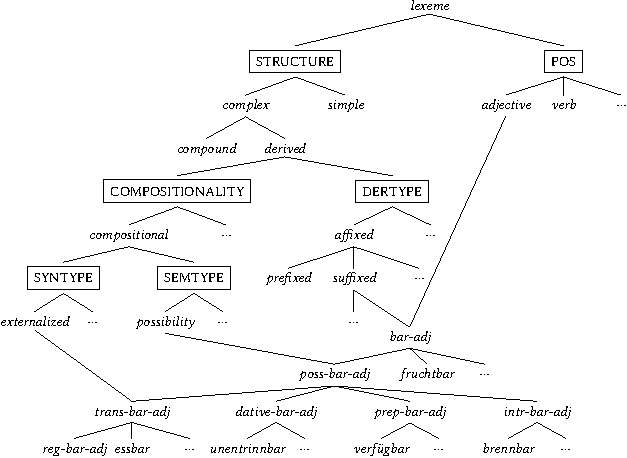
\includegraphics[scale=1.2]{figures/Riehemann-crop.pdf}

\bigskip

\begin{forest}
  type hierarchy
  [lexeme, for tree={s sep=0.1em},
    [structure, partition
      [complex
        [compound]
        [derived
          [compositionality, partition
            [compositional
              [syntype, partition
                [externalized, name=ext]
                [\ldots]
              ]
              [semtype, partition
                [possibility, name=poss]
                [\ldots]
              ]
            ]
            [noncomp]
          ]
          [dertype, partition
            [affixed
              [prefixed]
              [suffixed, name=suff]
            ]
            [\ldots]
          ]
        ]
      ]
      [simple]
    ]
    [pos, partition, calign=2
      [adjective
        [bar-adj, l*=6, calign=2, edge to=suff,
          [poss-bar-adj, calign children=23, edge to=poss,
            for children={s sep=0},
            [trans-bar-adj, calign=2, edge to=ext,
              [reg-bar-adj]
              [essbar]
              [\ldots]
            ]
            [dative-bar-adj
              [unentrinnbar]
              [\ldots]
            ]
            [prep-bar-adj
              [verfügbar]
              [\ldots]
            ]
            [intr-bar-adj
              [brennbar]
              [\ldots]
            ]
          ]
          [fruchtbar]
          [\ldots]
        ]
        [bar-adj, l*=6, phantom]
      ]
      [verb]
      [\ldots]
    ]
  ]
\end{forest}

Wow!

\newpage
\includegraphics[scale=.84]{figures/OTC-crop.pdf}

\newpage
  \includegraphics[scale=.63]{figures/pretyping-crop.pdf}


\newpage

\begin{forest}
[\emph{verb-infl}
	[2ND-SLOT,draw
    	[\emph{1sg},name=1sg
    		[\emph{1sg-pos}]
    	]
    	[\emph{3pl}]
   ]
	[1ST-SLOT,draw
		[\emph{neg}
			[\emph{1sg-neg},name=neg]
			[\emph{¬1sg-neg}]
		]
		[\emph{pos}]
	]
	[3RD-SLOT,draw
		[\emph{pst}
			[\emph{pos-pst}]
			[\emph{neg-pst}]
		]
		[\emph{fut}]
	]
]
\draw (1sg.south) to (neg.north);
\end{forest}

\bigskip

\begin{forest} type hierarchy
  [verb-infl, calign=2
    [2nd-slot,partition
      [1sg,name=1sg
        [1sg-pos]
      ]
      [3pl]
    ]
    [1st-slot,partition
      [neg
        [1sg-neg,edge to=!Pp] % Draw edge to ??? previous leaf (P) 
        [¬1sg-neg]
      ]
      [pos]
    ]
    [3rd-slot,partition
      [pst
        [pos-pst]
        [neg-pst]
      ]
      [fut]
    ]
  ]
\end{forest}

Stefan: What does ``Pp'' mean? Isn't P the previous leaf and p the previous sibling.

Sašo: Correct.

Stefan: But the previous leaf is 1sg-pos and it does not have a previous sibling.

Sašo: Incorrect. The previous leaf is ``3pl.''

\newpage

%% This does not compile ....

\scalebox{.8}{%
\begin{forest}for tree={l=2cm}
[\emph{realisation-rule}
	[MORPHOTACTICS,draw, name=morph
		[\avmtmp{
			[
			mud & \{\normalfont\textit{agr} \}\\
			ms & \{ [\type*{pid}
			cat & verb], ...\}\\
			mph & < [pc & $-4$]> ]
		}, name= 1, tier=word]
		[\avmtmp{
			[mud & \{\normalfont\textit{agr}\}\\
			 ms & \{ [\type*{pid}
			cat & [\type*{adj}
			type & A]], ...\}\\
			mph & < [pc & -1]>]
		}, name=2, tier=word]
	]
	[EXPONENCE,draw
		[QUAL,draw, name=qual
			[\avmtmp{
				[mud & \{ [\normalfont\textit{agr}\\cl & 7]\}\\
				mph & < ... [ph & <\normalfont ca>\\
				pc & $-1$ $\vee$ $-2$
				] ... >]
			}, tier=word]
			[\dots]
		]
		[CONC,draw, name=conc
			[\avmtmp{
				[mud & \{ [\normalfont\textit{agr}\\cl & 7]\}\\
				mph & < ... [ph & <\normalfont ci>\\
				pc & $-1$ $\vee$ $-4$
				] ... >]
			}, tier=word]
			[\dots]
		]
	]
]
%% sorry this is an ugly workaround but even on stackexchange, no one could help me :/
\node[below of=morph, node distance= 8cm](3){%
	\avmtmp{
			[mud & \{\normalfont\textit{agr}\}\\
			ms & \{ [\type*{pid}
			cat & [\type*{adj}
			type & B]], ...\}\\
			mph & <[pc & $-2$], [pc & $-1$]>]
	}%
};
\draw (1.north) to (qual.south);
\draw (2.north) to (conc.south);
\draw (3.north) to (morph.south);
\end{forest}
}    



\scalebox{.8}{%
\begin{forest}for tree={l=2cm}
[\emph{realisation-rule}
	[MORPHOTACTICS,draw, name=morph
		[\avmtmp{
			[
			mud & \{\normalfont\textit{agr} \}\\
			ms & \{ [\type*{pid}
			cat & verb], ...\}\\
			mph & < [pc & $-4$]> ]
		}, name= 1, tier=word]
		[\avmtmp{
			[mud & \{\normalfont\textit{agr}\}\\
			 ms & \{ [\type*{pid}
			cat & [\type*{adj}
			type & A]], ...\}\\
			mph & < [pc & -1]>]
		}, name=2, tier=word]
	]
	[EXPONENCE,draw
		[QUAL,draw, name=qual
			[\avmtmp{
				[mud & \{ [\normalfont\textit{agr}\\cl & 7]\}\\
				mph & < ... [ph & <\normalfont ca>\\
				pc & $-1$ $\vee$ $-2$
				] ... >]
			}, tier=word]
			[\dots]
		]
		[CONC,draw, name=conc
			[\avmtmp{
				[mud & \{ [\normalfont\textit{agr}\\cl & 7]\}\\
				mph & < ... [ph & <\normalfont ci>\\
				pc & $-1$ $\vee$ $-4$
				] ... >]
			}, tier=word]
			[\dots]
		]
	]
]
%% sorry this is an ugly workaround but even on stackexchange, no one could help me :/
%% saso: do you want to achieve the same as I did in \ref{trick-for-later}?
\node[below of=morph, node distance= 8cm](3){%
	\avmtmp{
			[mud & \{\normalfont\textit{agr}\}\\
			ms & \{ [\type*{pid}
			cat & [\type*{adj}
			type & B]], ...\}\\
			mph & <[pc & $-2$], [pc & $-1$]>]
	}%
};
\draw (1.north) to (qual.south);
\draw (2.north) to (conc.south);
\draw (3.north) to (morph.south);
\end{forest}
}    




\newpage

  \begin{tabular}{lcc}
    \rnode{u1}{\textsc{beak}} & \rnode{u2}{\textsc{gen}} & \rnode{u3}{\textsc{pl}}\\[2ex]
    \rnode{l1}{nokk} & \rnode{l2}{-a} & \rnode{l3}{-de}
  \end{tabular}
      \psset{angleA=-90,angleB=90,arm=0pt,linewidth=.5pt}

      \ncdiag{u1}{l1} \ncdiag{u1}{l2} \ncdiag{u2}{l1} \ncdiag{u2}{l3}
      \ncdiag{u3}{l1} \ncdiag{u3}{l2} \ncdiag{u3}{l3}

\bigskip

\begin{forest}
  [,phantom,
    for children={font=\sc},
    [beak
      [nokk, edge to=!r2, edge to=!r3]
    ]
    [gen
      [-a, edge to=!r1, edge to=!r3, no edge]
    ]
    [pl
      [-de, edge to=!r2]
    ]
  ]
\end{forest}

\newpage

\begin{forest}
[\emph{realisation-rule}
	[SHAPE,draw
		[\avmtmp{
			[ mph & \{[ph &  <\normalfont ni>]\}\\
			mud & \{[per & 1\\ num & sg]\}
			]
		}, name=1
			[\avmtmp{
				[ mph & \{[ph &  <\normalfont ni>\\ pc & 2]\}\\
				mud & \{ [\type*{subj} per & 1\\ num & sg] \}
				]
			}, name=a, no edge, tier=word, l=3cm]
		]
		[\avmtmp{
			[ mph & \{[ph &  <\normalfont wa>]\}\\
			mud & \{[per & 3\\ num & pl]\}
			]
		}, name=2
			[\avmtmp{
				[ mph & \{[ph &  <\normalfont wa>\\ pc & 5]\}\\
				mud & \{ [\type*{obj} per & 3\\ num & pl] \}
				]
			}, name=b, no edge, tier=word, l=3cm]
		]
	]
	[POSITION,draw
		[\avmtmp{
			[ mph & \{[pc & 2]\}\\
			mud & \{subj\}
			]
		}, name=3
			[\avmtmp{
				[ mph & \{[ph &  <\normalfont wa>\\ pc & 2]\}\\
				mud & \{ [\type*{subj} per & 3\\ num & pl] \}
				]
			}, name=c, no edge, tier=word, l=3cm]
		]
		[\avmtmp{
			[ mph & \{[pc & 5]\}\\
			mud & \{ obj \}
			]
		}, name=4
			[\avmtmp{
				[ mph & \{[ph &  <\normalfont ni>\\ pc & 5]\}\\
				mud & \{[\type*{obj} per & 1\\ num & sg]\}
				]
			}, name=d, no edge, tier=word, l=3cm]
		]
	]
]
\draw[dashed] (1.south) to (a.north);
\draw[dashed] (1.south) to (d.north);
\draw[dashed] (2.south) to (b.north);
\draw[dashed] (2.south) to (c.north);
\draw[dashed] (3.south) to (c.north);
\draw[dashed] (3.south) to (a.north);
\draw[dashed] (4.south) to (b.north);
\draw[dashed] (4.south) to (d.north);
\end{forest}






\end{document} 

%%%%%%%%%%%%%%%%%%%%%%%%%%%%%%%%%%%%%%%%%%%%%%%%%%%% 
%%%                  END                         %%% 
%%%%%%%%%%%%%%%%%%%%%%%%%%%%%%%%%%%%%%%%%%%%%%%%%%%% 

%%% Local Variables:
%%% mode: latex
%%% TeX-master: t
%%% TeX-engine: xetex
%%% End:
